\documentclass[a4paper,12pt]{article}
\usepackage[margin=22mm]{geometry}
\usepackage{fontspec}
\usepackage{polyglossia}
\setdefaultlanguage{ukrainian}
\setotherlanguage{english}
\setmainfont{STIXTwoText-Regular.otf}[
  BoldFont=STIXTwoText-Bold.otf,
  ItalicFont=STIXTwoText-Italic.otf,
  BoldItalicFont=STIXTwoText-BoldItalic.otf]
\newfontfamily\cyrillicfont{STIXTwoText-Regular.otf}[
  Script=Cyrillic,
  Ligatures=TeX,
  BoldFont=STIXTwoText-Bold.otf,
  ItalicFont=STIXTwoText-Italic.otf,
  BoldItalicFont=STIXTwoText-BoldItalic.otf]
\usepackage{amsmath,amssymb,booktabs}
\usepackage{etoolbox}
\usepackage{unicode-math}
\setmathfont{STIXTwoMath-Regular.otf}[Scale=1.0]
% \mathsf is a text-font alphabet in unicode-math (it would fall back to Latin Modern Sans); use the
% STIX Two Math sans-serif alphabet instead, so that only STIX Two fonts are embedded.
\AtBeginDocument{\let\mathsf\symsf}
% Keep vector/tensor notation bold italic; keep the zero vector bold upright.
\newcommand{\bm}[1]{\ifstrequal{#1}{0}{\symbf{#1}}{\symbfit{#1}}}
\usepackage{graphicx,placeins,needspace,microtype}
\usepackage{subcaption}
\captionsetup{font=small}
\captionsetup[subfigure]{font=small,skip=3pt,justification=raggedright}
\usepackage[numbers,square,sort&compress]{natbib}
\usepackage{xcolor}

\definecolor{referenceblue}{RGB}{25,55,95}
\usepackage[colorlinks,allcolors=referenceblue]{hyperref}
\providecommand{\doi}[1]{\href{https://doi.org/#1}{https://doi.org/#1}}
\setlength{\parindent}{1.4em}
\setlength{\emergencystretch}{1.5em}
\setlength{\textfloatsep}{14pt}
\renewcommand{\topfraction}{0.9}
\renewcommand{\bottomfraction}{0.8}
\renewcommand{\textfraction}{0.09}
\renewcommand{\floatpagefraction}{0.75}
\pdfstringdefDisableCommands{\def\texttt#1{#1}}
\newcommand{\qmix}{q_{\mathrm{K}}}
\newcommand{\dd}{\mathrm{d}}
% BEGIN AUDITED DATA: populated by sync_manuscript_data.py
% Snapshot: cfdf0f110010d688a4e3c48f6d88a00fd17dc698; no P24 physical data.
% Evidence JSON SHA256: db7c5908e2cad5c749c7914f4eb742b28d1d404b4124a03107f35b94ad013bd3
\newcommand{\PlateAMM}{300}
\newcommand{\PlateBMM}{100}
\newcommand{\HoleCxMM}{170}
\newcommand{\HoleCyMM}{-20}
\newcommand{\HoleRMM}{30}
\newcommand{\PhiStar}{-1.5606}
\newcommand{\MouthX}{0.199989}
\newcommand{\MouthY}{-0.0208170}
\newcommand{\NormalX}{0.999629}
\newcommand{\NormalY}{-0.0272345}
\newcommand{\PeakStress}{3.7141}
\newcommand{\LoadFactor}{80.774}
\newcommand{\LastXMM}{291.840}
\newcommand{\LastYMM}{-25.579}
\newcommand{\LSLengthMM}{84.15}
\newcommand{\LastLigamentMM}{8.16}
\newcommand{\MinimumTheta}{-3.646}
\newcommand{\MaxCODError}{0.01024}
\newcommand{\CODQuadMin}{0.6204}
\newcommand{\CODQuadMax}{0.6225}
\newcommand{\CODNearZeroPercent}{26.3}
\newcommand{\CODNearZeroTurnDiff}{0.00245}
\newcommand{\SyntheticRelativeError}{3.86\times10^{-8}}
\newcommand{\MaxTrueResidual}{1.00\times10^{-10}}
\newcommand{\CharacteristicRows}{$P_{1}$ & 4 & 0.36648 & $4.198\times10^{-6}$ & $1.146\times10^{-5}$ & 0.0000 & -0.00131 \\
$P_{17}$ & 68 & 0.78679 & $2.548\times10^{-3}$ & $3.239\times10^{-3}$ & -2.4444 & -0.37115 \\
$P_{21}$ & 84 & 0.96631 & $7.860\times10^{-5}$ & $8.134\times10^{-5}$ & -3.6366 & -0.00932 \\
$P_{22}$ & 88 & 1.0667 & $-2.284\times10^{-3}$ & $-2.142\times10^{-3}$ & -3.6460 & +0.24541 \\
$P_{23}$ & 92 & 1.2444 & $-6.780\times10^{-3}$ & $-5.449\times10^{-3}$ & -3.4006 & +0.62435 \\}
% END AUDITED DATA

\title{Покрокове визначення траєкторії поширення тріщини від контуру кругового отвору в рамках лінійної
механіки руйнування}
\author{Вячеслав Богданов, Данило Селіванов\\[4pt]
  \small Інститут механіки ім. С. П. Тимошенка НАН України, Київ}
\date{}
\hypersetup{pdftitle={Покрокове визначення траєкторії поширення тріщини від контуру кругового отвору в рамках лінійної
механіки руйнування},pdfauthor={Вячеслав Богданов, Данило Селіванов},pdflang={uk-UA}}
\begin{document}
\maketitle


\begin{abstract}
Визначення траєкторії поширення тріщини, що зароджується на контурі кругового отвору, потребує встановлення зв’язку між станом зародження та послідовністю розв’язків для вершини тріщини за змішаного навантаження. Задачу розглянуто в квазістатичній постановці лінійної механіки
руйнування. Точку зародження вибирають за максимумом розтягувального колового напруження на контурі отвору. Першу ланку спрямовано вздовж нормалі від отвору в матеріал. Напрями наступних
ланок визначають за критерієм максимальних колових напружень із використанням коефіцієнтів
інтенсивності напружень (КІН), обчислених за інтегралом взаємодії для повної поточної геометрії
тріщини. Способи обчислення цих коефіцієнтів і вибору напряму оцінено за допомогою заданих
полів, порівняння з оцінками за переміщеннями розкриття тріщини та перевірки симетрії на
пластині з центральним отвором. Чутливість траєкторії оцінено за незалежними розрахунками
поширення зі зміненими зовнішньою та структурованою привершинною сітками. Для отвору, зміщеного відносно центра пластини, відношення КІН з урахуванням знака сягає додатного максимуму, а згодом змінює знак.
Напрям покрокового повороту при цьому змінюється на протилежний, а коефіцієнт інтенсивності
напружень нормального відриву далі зростає за незмінного віддаленого навантаження. Для незалежно
обчислених траєкторій із приростами 4, 2 і 1 мм, за одночасного зменшення характерних
розмірів дискретизації, різниці координат і напрямів зменшуються, а кути повороту, віднесені до приросту довжини, майже не змінюються. Характерна послідовність поворотів зберігається за
досліджених змін сітки. Одночасне зменшення приросту довжини тріщини та масштабів дискретизації виявляє тенденції зміни змішаності мод та
інтенсивності повороту без виокремлення впливу приросту довжини.
\end{abstract}
\noindent\textbf{Ключові слова.} траєкторія поширення тріщини, круговий отвір, лінійна механіка руйнування, критерій максимальних
колових напружень, змішаність мод деформування, інтеграл взаємодії

\section{Вступ}
Отвори в елементах конструкцій є концентраторами напружень, на контурі яких можуть зароджуватися тріщини.
Для оцінки міцності таких елементів важливо визначити не лише умови зародження тріщини, а й траєкторію її подальшого поширення.
Визначенню коефіцієнтів інтенсивності напружень (КІН) для радіальних і похилих тріщин, що виходять із контуру кругового отвору,
присвячено низку праць~\cite{Bowie1956,WooWangCheung1989,XuEtAl2018}.
Умови зародження тріщин біля отворів та стійкість їх подальшого поширення досліджено також у рамках механіки руйнування
зі скінченним приростом тріщини~\cite{SaporaEtAl2018,SaporaCornetti2018}.
Однак визначення місця зародження тріщини є лише початковим етапом побудови її траєкторії.

У рамках лінійної механіки руйнування (LEFM) одним із поширених підходів до визначення напряму поширення тріщини
є застосування критерію максимальних колових напружень (MTS), запропонованого Ердоганом і Сі~\cite{ErdoganSih1963}.
Цей критерій дає змогу визначити напрям поширення тріщини за коефіцієнтами інтенсивності напружень нормального відриву
та поперечного зсуву, відповідно $K_{\mathrm I}$ і $K_{\mathrm{II}}$.
Для моделювання поширення тріщин застосовують різні чисельні методи, зокрема метод скінченних елементів,
метод граничних елементів та розширений ізогеометричний аналіз~\cite{BouchardEtAl2003,LiuLiXie2017,FangEtAl2020,AlshoaibiFageehi2022}.

Особливістю задачі визначення траєкторії поширення тріщини є взаємозалежність її геометрії та напружено-деформованого стану
в околі вершини. Зміна конфігурації тріщини впливає на співвідношення коефіцієнтів інтенсивності напружень,
від якого, своєю чергою, залежить напрям її подальшого поширення.
У зв’язку з цим особливого значення набуває точність визначення коефіцієнта інтенсивності напружень поперечного зсуву,
зокрема коли його значення є малим порівняно з коефіцієнтом інтенсивності напружень нормального відриву.
За таких умов чисельна асиметрія дискретизації в околі вершини може істотно впливати на визначення локального напряму поширення тріщини.
Це ускладнює, зокрема, дослідження зміни траєкторії під час наближення тріщини до межі тіла.

Метою цієї роботи є визначення траєкторії поширення тріщини, що зароджується на контурі кругового отвору,
зміщеного відносно центра пластини, та дослідження закономірностей зміни коефіцієнтів інтенсивності напружень у процесі її поширення.
Для підвищення точності визначення зсувного коефіцієнта інтенсивності напружень використано структуровану скінченно-елементну сітку
з попарно дзеркально симетричним розташуванням елементів відносно останньої ланки тріщини в околі її вершини.
Особливу увагу приділено взаємозв’язку між співвідношенням коефіцієнтів інтенсивності напружень, напрямом повороту тріщини
та приростом її довжини. Достовірність отриманих результатів оцінено шляхом зіставлення різних способів визначення
коефіцієнтів інтенсивності напружень і дослідження чутливості розрахованої траєкторії до параметрів дискретизації.

\section{Постановка задачі}
\label{sec:problem}
Розглянемо прямокутну пластину шириною $2A=\PlateAMM$ мм і висотою $B=200$ мм із круговим отвором
радіуса $R=\HoleRMM$ мм (рис.~\ref{fig:geometry-loading}). Координати центра отвору відносно лівого нижнього
кута пластини становлять $x_{\mathrm c}=170$ мм, $y_{\mathrm c}=80$ мм. Початок розрахункової декартової
системи координат $Oxy$ розташовано посередині лівого краю пластини, вісь $x$ спрямовано праворуч,
а вісь $y$ --- вгору.

Матеріал пластини однорідний, ізотропний, лінійно-пружний, з модулем Юнга $E=210$ ГПа та коефіцієнтом
Пуассона $\nu=0.30$. Модуль зсуву $\mu=E/[2(1+\nu)]$. Розглядаємо плоску деформацію. До верхнього та нижнього країв пластини прикладено
рівномірне розтягувальне навантаження інтенсивності $\sigma>0$, спрямоване назовні.
Вертикальні краї пластини, контур отвору та береги тріщини вільні від навантаження.
Переміщення тіла як цілого усунуто закріпленням обох компонент переміщень у лівому нижньому куті
та вертикальної компоненти у правому нижньому куті. Об’ємні сили відсутні.

\begin{figure}[htbp]
  \centering
  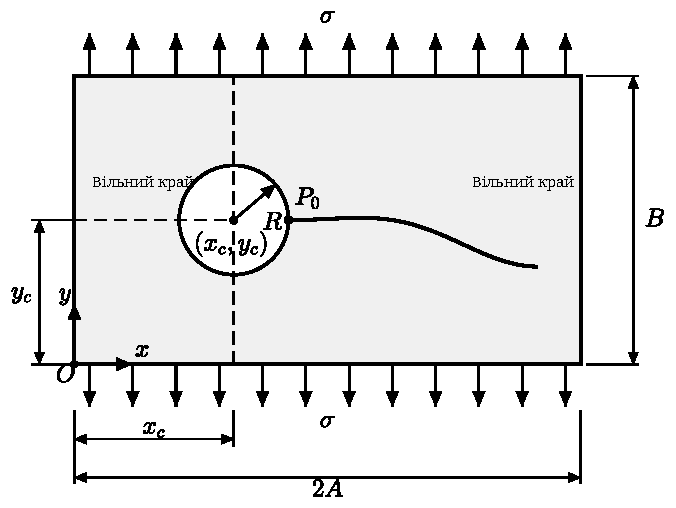
\includegraphics[width=0.78\textwidth]{figures/geometry_loading/specimen_geometry.pdf}
  \caption{Геометрія пластини з круговим отвором, схематичне зображення траєкторії тріщини та прикладене навантаження.
  Координати центра отвору $(x_{\mathrm c},y_{\mathrm c})$ відлічено від лівого нижнього кута пластини. Розміри подано без дотримання масштабу.}
  \label{fig:geometry-loading}
\end{figure}

На першому етапі розв’язуємо задачу теорії пружності для пластини з отвором без тріщини.
Точку зародження тріщини вибираємо на контурі отвору в місці максимального розтягувального
колового нормального напруження $\sigma_{tt}$. Кутове положення цієї точки визначаємо за умовою
\begin{equation}
 \phi_*=\mathop{\operatorname{arg\,max}}_\phi\sigma_{tt}^{+}(\phi),
 \qquad
 \sigma_{tt}^{+}=\max(\sigma_{tt},0).
 \label{eq:initiation}
\end{equation}
Тут кут $\phi$ відлічуємо від додатного напряму осі $x$ проти годинникової стрілки.
Координати точки зародження $P_0$ у розрахунковій системі координат та одиничний вектор нормалі
до контуру отвору, спрямованої в матеріал, визначаємо співвідношеннями
\begin{equation}
 P_0=\begin{bmatrix}x_{\mathrm c}+R\cos\phi_*\\
                     y_{\mathrm c}-B/2+R\sin\phi_*
     \end{bmatrix},
 \qquad
 \bm n_{\mathrm{mat}}=\begin{bmatrix}\cos\phi_*\\\sin\phi_*\end{bmatrix}.
 \label{eq:mouth}
\end{equation}

Розрахунки виконуємо за еталонного навантаження $\sigma=1$ МПа. За пропорційного збільшення навантаження
обидва КІН змінюються в однаковій пропорції, тому їхнє відношення, а отже, і визначений за критерієм MTS
напрям поширення тріщини не залежать від величини навантаження.

Траєкторію тріщини апроксимуємо ламаною, що складається з прямолінійних ланок довжини $\Delta a$.
Першу ланку спрямовуємо вздовж нормалі до контуру отвору в точці зародження:
\begin{equation}
 P_1=P_0+\Delta a\,\bm n_{\mathrm{mat}}.
 \label{eq:first}
\end{equation}
Для опису траєкторії використовуємо фіксований ортонормований базис $(\bm n_{\mathrm{mat}},\bm t)$,
де $\bm t=(-n_{\mathrm{mat},y},n_{\mathrm{mat},x})^{\mathsf T}$. Кути нахилу ланок $\theta_k$ відлічуємо
від напряму $\bm n_{\mathrm{mat}}$, тому $\theta_1=0$. Напрями всіх наступних ланок визначаємо
в процесі розв’язання задачі. На кроці $k$ область матеріалу $\Omega_k$ обмежена зовнішнім контуром
пластини, контуром отвору та берегами тріщини $\Gamma_k$ з вершиною $P_k$.

Розглядаємо квазістатичне поширення однієї тріщини із заданими приростами її довжини.
Критичні навантаження при зародженні та подальшому поширенні, конкурентне зародження інших тріщин
і умови зупинки тріщини в цій роботі не досліджуємо.

\section{Покрокова побудова траєкторії поширення тріщини}
\label{sec:recurrence}
\subsection{Коефіцієнти інтенсивності напружень}
На кожному кроці розв’язуємо задачу теорії пружності з урахуванням усієї сформованої геометрії тріщини.
У поточній вершині $P_k$ вводимо локальну декартову систему координат, вісь $x_1$ якої спрямована
вздовж останньої ланки тріщини. Одиничні вектори локального базису визначаємо співвідношеннями
\[
 \bm e_1^{(k)}=\frac{P_k-P_{k-1}}{\Delta a},
 \qquad
 \bm e_2^{(k)}=\begin{bmatrix}-e_{1y}^{(k)}\\e_{1x}^{(k)}\end{bmatrix}.
\]
Коефіцієнти інтенсивності напружень нормального відриву та поперечного зсуву в поточній вершині тріщини становлять
\begin{equation}
 \begin{aligned}
 K_{\mathrm I}^{(k)}&=\lim_{r\to0^+}\sqrt{2\pi r}\,\sigma_{22}(r,0),\\
 K_{\mathrm{II}}^{(k)}&=\lim_{r\to0^+}\sqrt{2\pi r}\,\sigma_{12}(r,0),
 \end{aligned}
 \label{eq:sifdefinition}
\end{equation}
де $r$ --- відстань від вершини тріщини вздовж додатного напряму осі $x_1$,
а компоненти тензора напружень визначено в локальній системі координат.

Для характеристики змішаності мод деформування використовуємо безрозмірний коефіцієнт
\begin{equation}
 q_{\mathrm K}^{(k)}=\frac{K_{\mathrm{II}}^{(k)}}{K_{\mathrm I}^{(k)}},
 \qquad K_{\mathrm I}^{(k)}>0.
 \label{eq:mode-mixity}
\end{equation}
Знак цього коефіцієнта збігається зі знаком зсувного КІН.

\subsection{Визначення напряму поширення тріщини}
Напрям нової ланки визначаємо за критерієм максимальних колових напружень.
Кут повороту $\alpha$ відносно попередньої ланки, додатний проти годинникової стрілки, задовольняє рівняння
\begin{equation}
 K_{\mathrm I}^{(k)}\sin\alpha+
 K_{\mathrm{II}}^{(k)}(3\cos\alpha-1)=0.
 \label{eq:mts-angle}
\end{equation}
Для розглянутих станів із додатним КІН нормального відриву потрібний корінь відповідає максимуму
розтягувального колового напруження та неперервно переходить у нуль за зникнення зсувного КІН.

За малої змішаності мод розклад розв’язку цього рівняння має вигляд
\begin{equation}
 \alpha_{\mathrm{MTS}}
 =-2q_{\mathrm K}^{(k)}
 +\frac{14}{3}\bigl(q_{\mathrm K}^{(k)}\bigr)^3
 +O\bigl((q_{\mathrm K}^{(k)})^5\bigr),
 \label{eq:mts-small-mixity}
\end{equation}
де кут виражено в радіанах. Отже, додатному зсувному КІН відповідає поворот тріщини за годинниковою
стрілкою, а від’ємному --- проти годинникової стрілки.
Це наближення використовуємо для інтерпретації результатів. Під час побудови траєкторії розв’язуємо
рівняння критерію MTS без зазначеного наближення.

\subsection{Побудова траєкторії}
Одиничний вектор, що визначає напрям ланки тріщини у фіксованому базисі, має вигляд
\begin{equation}
 \bm e(\theta)=\cos\theta\,\bm n_{\mathrm{mat}}+\sin\theta\,\bm t.
 \label{eq:direction}
\end{equation}
Кут повороту, кут нахилу нової ланки та положення нової вершини визначаємо послідовно:
\begin{align}
 \Delta\theta_{k+1}&=\alpha_{\mathrm{MTS}},\label{eq:turn}\\
 \theta_{k+1}&=\theta_k+\Delta\theta_{k+1},\label{eq:angleupdate}\\
 P_{k+1}&=P_k+\Delta a\,\bm e(\theta_{k+1}).\label{eq:pointupdate}
\end{align}
Таким чином, напрям кожної наступної ланки залежить від напруженого стану, зумовленого всією
попередньо сформованою геометрією тріщини. Довжину тріщини відраховуємо від точки її зародження: $a_k=k\Delta a$.

Для характеристики зміни напряму поширення тріщини використовуємо інтенсивність повороту ---
відношення кута повороту до приросту її довжини:
\[
 \frac{\Delta\theta_{k+1}}{\Delta a}.
\]
Якщо за зменшення приросту довжини тріщини розраховані траєкторії наближаються до гладкої кривої,
а наведене відношення збігається до її знакової кривини, то з асимптотичного розкладу критерію MTS
випливає співвідношення
\begin{equation}
 \frac{q_{\mathrm K}^{(k)}}{\Delta a}
 =-\frac12\frac{\Delta\theta_{k+1}}{\Delta a}
  +O((\Delta a)^2)
 \longrightarrow-\frac12\frac{\dd\theta}{\dd a}.
 \label{eq:curvature-mts}
\end{equation}
Тут $\theta$ --- кут нахилу дотичної до гладкої кривої, параметризованої довжиною дуги $a$.
Отже, за зазначених умов відношення коефіцієнта змішаності мод до приросту довжини тріщини
характеризує кривину її траєкторії з урахуванням знака.
Самої збіжності координат точок траєкторії для цього недостатньо.

\section{Чисельна реалізація та верифікація}
\label{sec:numerics}
\subsection{Скінченно-елементна дискретизація}
\label{sec:numerical-parameters}
Для розв’язання задачі використовуємо шестивузлові трикутні скінченні елементи (T6) з квадратичною
апроксимацією переміщень. Для пластини без тріщини контур отвору апроксимуємо багатокутником із 480 сторонами.
Колові нормальні напруження на контурі визначаємо лінійною екстраполяцією значень,
обчислених у матеріалі на трьох відстанях від контуру. Локальна квадратична апроксимація
розподілу цих напружень за кутовою координатою дає положення точки їх максимуму
\[
 \phi_*=\PhiStar^\circ.
\]
Точку зародження тріщини та напрям першої ланки визначаємо за цим кутом.

На кожному кроці поширення тріщини перебудовуємо сітку відповідно до її нової геометрії.
Для цього до області отвору приєднуємо вузький допоміжний виріз уздовж усієї ламаної тріщини.
Після тріангуляції області протилежні краї вирізу суміщаємо з лінією тріщини, зберігаючи
роздільність вузлів її берегів. Аналогічний підхід до побудови сітки
використано в задачі про поворот тріщини в рамках моделі когезійної зони~\cite{BogdanovSelivanov2026}.
Тривузлові трикутники (T3) перетворюємо на елементи T6 із прямолінійними сторонами.

Для підвищення точності визначення зсувного КІН в околі вершини тріщини будуємо структуровану сітку,
елементи якої попарно дзеркально симетричні відносно останньої ланки тріщини (рис.~\ref{fig:mesh-levels}).
За межами цієї області використовуємо узгоджену неструктуровану сітку з поступовим збільшенням
розмірів елементів у міру віддалення від вершини. Радіус структурованої області позначимо через
$r_{\mathrm{core}}$, а характерний крок сітки в ній --- через $h_{\mathrm{tip}}$.
Для основного варіанта розрахунку з приростом довжини тріщини 4 мм маємо
\[
 r_{\mathrm{core}}=3\ \text{мм},\qquad h_{\mathrm{tip}}=h_0=0.027012\ \text{мм}.
\]
На рис.~\ref{fig:mesh-levels} наведено скінченно-елементну сітку, побудовану для отриманої
траєкторії тріщини при її довжині 84 мм. На рис.~\ref{fig:mesh-core} сірим кольором виділено
елементи зі змінною ваговою функцією інтеграла взаємодії. На рис.~\ref{fig:mesh-symmetry}
показано три пари дзеркально симетричних елементів. Вузли протилежних берегів тріщини мають
однакові координати, але різну нумерацію (позначено колами), тоді як вузли перед вершиною
є спільними для елементів обох половин структурованої області (позначено точками).
На рисунку наведено лише кутові вузли елементів T6.

\begin{figure}[tbp]
  \centering
  \begin{minipage}{\textwidth}
  \centering
  \begin{subfigure}[t]{0.485\linewidth}
    \centering
    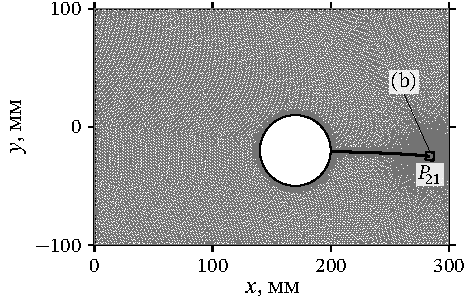
\includegraphics[width=\linewidth]{figures/iam_f02/a_global_mesh.pdf}
    \caption{Сітка всієї пластини.}
    \label{fig:mesh-global}
  \end{subfigure}\hfill
  \begin{subfigure}[t]{0.485\linewidth}
    \centering
    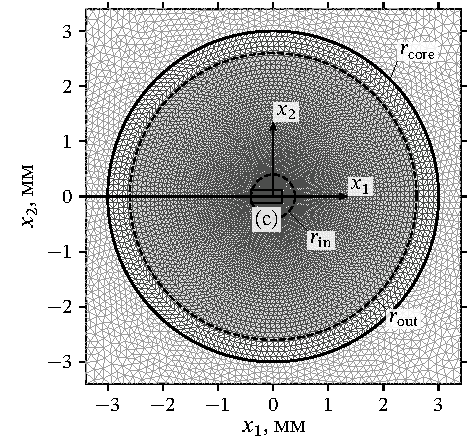
\includegraphics[width=\linewidth]{figures/iam_f02/b_structured_region.pdf}
    \caption{Структурована привершинна область.}
    \label{fig:mesh-core}
  \end{subfigure}

  \vspace{4pt}
  \begin{subfigure}[t]{0.94\linewidth}
    \centering
    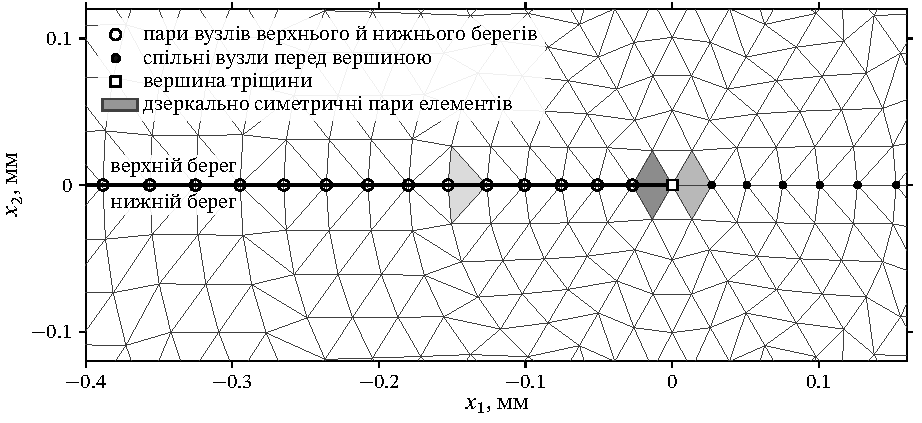
\includegraphics[width=\linewidth]{figures/iam_f02/c_symmetry_detail.pdf}
    \caption{Дзеркальна симетрія сітки біля вершини.}
    \label{fig:mesh-symmetry}
  \end{subfigure}
  \end{minipage}
  \caption{Скінченно-елементна сітка для тріщини довжини 84 мм:
  (a) загальна сітка пластини; (b) структурована привершинна область та область інтегрування;
  (c) дзеркально симетричні елементи й вузли берегів тріщини.}
  \label{fig:mesh-levels}
\end{figure}

На кожному кроці поширення тріщини перевіряємо виконання умов геометричної та топологічної
допустимості скінченно-елементної сітки. Контролюємо збереження геометрії тріщини та меж області,
роздільність вузлів берегів тріщини, спільність вузлів перед її вершиною, дзеркальну симетрію
привершинних елементів і узгодженість структурованої та неструктурованої сіток.
Структурована область не має перетинати контур отвору чи зовнішній контур пластини,
а попередня вершина тріщини має перебувати за її межами. Область інтегрування має цілком
міститися в структурованій області. Перевіряємо також додатність площ трикутників
і якобіанів перетворення координат. У зоні перебудови сітки мінімальний кут трикутника
має становити не менше $20^\circ$, а відношення довжин найдовших сторін сусідніх
трикутників не має перевищувати 1.8. До розв’язання крайової задачі переходимо лише
за виконання встановлених умов допустимості сітки.

Вплив кроку привершинної сітки на КІН досліджуємо для заданих конфігурацій тріщини,
варіюючи крок сітки ($2h_0$, $h_0$, $h_0/2$) за незмінних радіусів структурованої області
та області інтегрування. Закон зміни розмірів зовнішніх елементів залишається незмінним,
проте їхню зв’язність узгоджуємо з новою привершинною сіткою. Для оцінювання впливу
дискретизації на траєкторію порівнюємо результати незалежних розрахунків із кроками $h_0$
і $2h_0$ до довжини тріщини 92 мм.

Вплив дискретизації поза структурованою областю досліджуємо за двох законів зміни розмірів
елементів (M0 і M1), для яких максимальні задані розміри елементів у віддаленій від вершини
області становлять відповідно 2.5 і 5 мм. Порівнюємо КІН за однакової геометрії тріщини,
а також траєкторії, отримані незалежно для кожного із цих законів. Основний варіант
розрахунку відповідає закону M0.

Крім того, розглядаємо траєкторії, незалежно визначені для приростів довжини тріщини 4, 2 та 1 мм.
У цих розрахунках відносний крок привершинної сітки вдвічі більший, ніж в основному
варіанті, а розміри зовнішніх елементів визначає закон M1. Характерні розміри структурованої
та зовнішньої сіток, а також радіуси області інтегрування пропорційні приросту довжини тріщини.
Тому зіставлення траєкторій характеризує спільний вплив приросту довжини тріщини
та дискретизації. Параметри дискретизації наведено в додатку~\ref{app:numerical-details}.

\subsection{Визначення КІН за інтегралом взаємодії}
Коефіцієнти інтенсивності напружень визначаємо за інтегралом взаємодії~\cite{YauWangCorten1980},
представленим у формі еквівалентного інтеграла за областю (EDI):
\begin{equation}
 I^{(m)}=\int_{\Omega_k}
 \left[-(\bm\sigma^{(m)}\!:\bm\varepsilon)\delta_{1j}
 +\sigma_{ij}u^{(m)}_{i,1}
 +\sigma^{(m)}_{ij}u_{i,1}\right]w_{,j}\,\dd\Omega.
 \label{eq:interaction}
\end{equation}
Верхній індекс у дужках відповідає допоміжному асимптотичному полю чистої моди I або II;
величини без цього індексу характеризують поле, отримане з розв’язку крайової задачі. Компоненти тензорів
і векторів визначено в локальній системі координат вершини тріщини. За повторюваними індексами
(від 1 до 2) виконуємо підсумовування, $\delta_{1j}$ --- символ Кронекера, кома з індексом
позначає частинну похідну, двокрапка --- згортку тензорів.

Значення радіальної вагової функції $w$ у вузлах сітки задаємо залежно від їхньої
відстані до вершини тріщини: функція дорівнює одиниці всередині круга радіуса $r_{\mathrm{in}}$,
лінійно спадає до нуля в кільцевій області та дорівнює нулю за межами круга радіуса $r_{\mathrm{out}}$.
Градієнт функції обчислюємо за її інтерполяцією в елементі T6.
Радіуси області інтегрування визначаємо співвідношеннями
\[
 r_{\mathrm{in}}=0.10\Delta a,\qquad r_{\mathrm{out}}=0.65\Delta a.
\]
Таким чином, область інтегрування розташована всередині структурованої привершинної області
(рис.~\ref{fig:mesh-core}).

В умовах плоскої деформації коефіцієнти інтенсивності напружень визначаємо зі співвідношень
\begin{equation}
 K_m=\frac{E'}{2K_{\mathrm{aux}}}I^{(m)},\qquad
 E'=\frac{E}{1-\nu^2},\qquad m\in\{\mathrm I,\mathrm{II}\},
 \label{eq:normalization}
\end{equation}
де $K_{\mathrm{aux}}$ --- КІН допоміжного поля, що в розрахунках дорівнює одиниці.

\subsection{Визначення КІН за переміщеннями берегів тріщини}
\label{sec:cod-extraction}
Для зіставлення з результатами визначення КІН за інтегралом взаємодії використовуємо також
метод екстраполяції переміщень берегів тріщини (COD)~\cite{GuineaPlanasElices2000}.
Дзеркальна симетрія привершинної сітки дає змогу використовувати пари вузлів T6 на протилежних
берегах останньої ланки тріщини, розташовані на однаковій відстані від її вершини.
За переміщеннями цих вузлів визначаємо наближені значення КІН на скінченній відстані від вершини:
\begin{equation}
 \begin{bmatrix}K_{\mathrm I}^{\mathrm{app}}(r)\\K_{\mathrm{II}}^{\mathrm{app}}(r)\end{bmatrix}
 =\frac{\mu}{\kappa+1}\sqrt{\frac{2\pi}{r}}
 \begin{bmatrix}{[\![u_2]\!]}\\{[\![u_1]\!]}\end{bmatrix},
 \qquad \kappa=3-4\nu.
 \label{eq:cod}
\end{equation}
Тут подвійними квадратними дужками позначено стрибки компонент переміщень (значення
на верхньому березі мінус значення на нижньому), $r$ --- відстань від вершини до пари вузлів
на останній ланці, $\kappa$ --- стала Колосова для плоскої деформації.

Для визначення КІН отримані значення апроксимуємо лінійними та квадратичними функціями
нормованої відстані від вершини з подальшою екстраполяцією до нуля. Для нормованої відстані $r/\Delta a$ розглядаємо чотири інтервали апроксимації:
\[
 [0.04,0.20],\quad [0.04,0.30],\quad [0.08,0.30],\quad [0.12,0.30].
\]
Поєднання двох видів апроксимації та чотирьох інтервалів дає вісім оцінок кожного КІН.
Оскільки обидва способи визначення КІН ґрунтуються на одному скінченно-елементному розв’язку,
їх зіставлення характеризує чутливість результатів до способу визначення КІН, але не забезпечує
незалежної оцінки похибки скінченно-елементного розв’язку. Під час побудови траєкторій використовуємо
КІН, визначені за інтегралом взаємодії.

\subsection{Верифікація чисельного методу}
Точність обчислення КІН за заданим полем переміщень оцінюємо на основі асимптотичних
розв’язків для чистих мод I та II, а також для змішаного деформування з відношенням
зсувного КІН до КІН нормального відриву, що дорівнює $10^{-4}$.
Найбільша відносна похибка визначення КІН для випадку малої змішаності мод на основних
сітках становить $\SyntheticRelativeError$. Ця оцінка не охоплює похибку
скінченно-елементного розв’язку крайової задачі.

Для перевірки відтворення симетрії напружено-деформованого стану розглянемо пластину з центральним
круговим отвором та радіальною тріщиною довжини 8 мм, що виходить із крайньої правої точки отвору.
За симетрії геометрії та навантаження зсувний КІН дорівнює нулю. Чисельно отримано
\[
 K_{\mathrm I}=0.42541\ \text{МПа}\sqrt{\text{м}},\qquad
 q_{\mathrm K}=6.22\times10^{-9}.
\]
Відповідний кут повороту наступної ланки за критерієм MTS становить
\[
 \alpha_{\mathrm{MTS}}=-7.13\times10^{-7}\ \text{градуса}.
\]
Мале значення зсувного КІН у цій задачі свідчить про точність чисельного відтворення
симетрії поля. Проте воно не визначає похибку ненульового зсувного КІН у несиметричній задачі.

Додатково досліджуємо реакцію напряму поширення тріщини на мале геометричне збурення.
Першу ланку завдовжки 4 мм залишаємо на лінії симетрії, а другу ланку такої самої довжини
відхиляємо від неї на заданий кут $\theta_2$, що набуває значень $\pm0.05^\circ$ та $\pm0.10^\circ$.
Для кожної конфігурації розв’язуємо крайову задачу, визначаємо КІН у вершині другої ланки
та за критерієм MTS обчислюємо кут повороту і кут нахилу третьої ланки:
\[
 \Delta\theta_3=\alpha_{\mathrm{MTS}},\qquad
 \theta_3=\theta_2+\Delta\theta_3.
\]
Кути нахилу обох ланок відлічуємо від лінії симетрії. Наприклад, для другої ланки з кутом
нахилу $+0.10^\circ$ кут повороту становить $-0.111415^\circ$, а кут нахилу третьої ланки
--- $-0.011415^\circ$. Для всіх розглянутих ненульових збурень нахил третьої ланки має
протилежний знак, а його абсолютна величина приблизно у 8.8 раза менша за абсолютну величину
заданого кута нахилу другої ланки. Отже, напрям поширення тріщини наближається до напряму
лінії симетрії зі зміною знака відхилення. Цей результат характеризує реакцію на збурення
на одному кроці й не встановлює стійкості всієї траєкторії.

Параметри сіток, спосіб розв’язання системи рівнянь методу скінченних елементів
та кількісні результати перевірок наведено в додатку~\ref{app:numerical-details}.
\FloatBarrier

\section{Результати розрахунку траєкторії поширення тріщини}
\label{sec:results}
\subsection{Прийнята траєкторія та зміна напряму}
Задана радіальна ланка $P_0P_1$ утворює початкову конфігурацію тріщини. За одиничного еталонного
навантаження її КІН нормального відриву та поперечного зсуву становлять відповідно $K_{\mathrm{I}}^{(1)}=0.36648$ і $K_{\mathrm{II}}^{(1)}=4.1983\times10^{-6}$
МПа$\sqrt{\text{м}}$. Малий додатний коефіцієнт змішаності мод дає початкову поправку за годинниковою стрілкою,
$\Delta\theta_2=\theta_2=-0.0013127^\circ$. Кожний наступний прийнятий напрям визначають із нового розв’язку пружної задачі. Так
одержано послідовність до $P_{23}$ включно.

На рис.~\ref{fig:trajectory} показано отриману ламану $P_0$--$P_{23}$, де суцільна лінія позначає прийняту геометрію
тріщини. Її загальна прийнята довжина становить 92 мм. Кінцева вершина та залишкова відстань до
правого краю по горизонталі становлять
\begin{equation}
 P_{23}=(\LastXMM,\LastYMM)\ \text{мм},\qquad
 2A-x_{23}=\LastLigamentMM\ \text{мм}.
\end{equation}
Наступну пробну ланку $P_{23}P_{24}$ показано штриховою лінією. Її геометрія пройшла перевірки, але для
пружної задачі у вершині $P_{24}$ не виконано критерій прийнятності.

Спочатку ламана повертає за годинниковою стрілкою. Модуль її від’ємного кута нахилу зростає.
Напрям ланки сягає $\theta_{22}=\MinimumTheta^\circ$ і стає менш від’ємним у $P_{23}$ (рис.~\ref{fig:intensities}). Ця зміна відображає додатний
покроковий поворот, без зміни напряму руху по вертикалі. Остання прийнята ланка й далі
спрямована нижче горизонталі. Траєкторія є кусково-лінійною. Неперервну криволінійну траєкторію
окремо не обчислювали.

\begin{figure}[tbp]
  \centering
  \begin{minipage}{0.8\textwidth}
  \centering
  \begin{subfigure}[t]{0.94\linewidth}
    \centering
    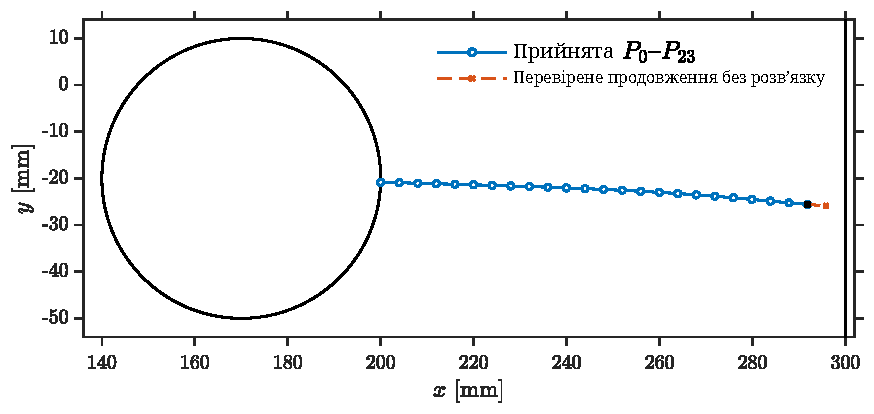
\includegraphics[width=\linewidth]{figures/trajectory/overview.pdf}
    \caption{Прийнята траєкторія та запропоноване продовження.}
    \label{fig:trajectory-overview}
  \end{subfigure}

  \medskip

  \begin{subfigure}[t]{0.94\linewidth}
    \centering
    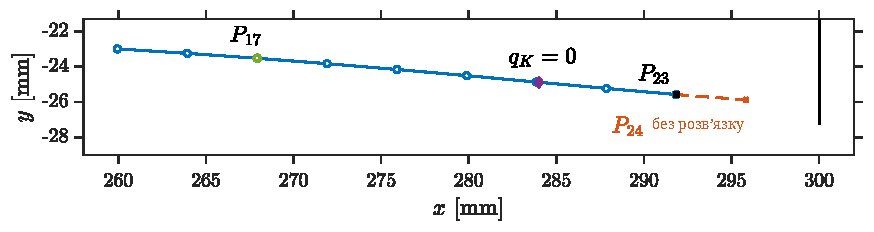
\includegraphics[width=\linewidth]{figures/trajectory/late_detail.pdf}
    \caption{Кінцева ділянка траєкторії та характерні точки.}
    \label{fig:trajectory-late}
  \end{subfigure}

  \end{minipage}
  \caption{Траєкторія поширення тріщини від контуру отвору, зміщеного відносно центра пластини. На кожній панелі горизонтальний і
вертикальний масштаби однакові. Суцільна лінія закінчується в останній прийнятій вершині $P_{23}$. Для
штрихового продовження $P_{23}P_{24}$ прийнятого пружного розв’язку немає. Ромб позначає інтерпольований
нуль коефіцієнта змішаності мод, а не вершину, для якої розв’язано задачу.}
  \label{fig:trajectory}
\end{figure}


\subsection{Зміна коефіцієнтів інтенсивності напружень і змішаності мод}
КІН нормального відриву монотонно зростає вздовж прийнятої траєкторії з приростом 4 мм від $K_{\mathrm{I}}=0.36648$ у
$P_1$ до $1.2444$ у $P_{23}$ (рис.~\ref{fig:intensities}). Усі ці значення обчислено за того самого одиничного віддаленого
навантаження. Зростання відображає зміну геометрії пружної задачі без зміни прикладеного
навантаження.

КІН поперечного зсуву спочатку близький до нуля і сягає найбільшого додатного значення $K_{\mathrm{II}}=0.0025484$ у $P_{17}$
($a=68$ мм). У тому самому стані коефіцієнт змішаності мод із рівняння~\eqref{eq:mode-mixity} сягає додатного
максимуму $q_{\mathrm{K}}=0.0032389$. Це максимум знакової величини, оскільки модуль від’ємного КІН поперечного зсуву в
останній прийнятій вершині більший. Максимум $|K_{\mathrm{II}}|$ припадає на інший стан. Після $P_{17}$ величина $K_{\mathrm{II}}$
зменшується, а $K_{\mathrm{I}}$ далі зростає. Зменшення додатного коефіцієнта змішаності мод зменшує модуль
повороту за MTS за годинниковою стрілкою до $P_{21}$ включно (рис.~\ref{fig:late}).

\begin{figure}[tbp]
  \centering
  \begin{minipage}{\textwidth}
  \centering
  \begin{subfigure}[t]{0.315\linewidth}
    \centering
    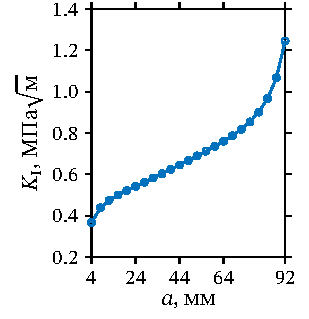
\includegraphics[width=\linewidth]{figures/intensities/KI.pdf}
    \caption{КІН нормального відриву $K_{\mathrm{I}}$.}
    \label{fig:intensities-KI}
  \end{subfigure}\hfill
  \begin{subfigure}[t]{0.315\linewidth}
    \centering
    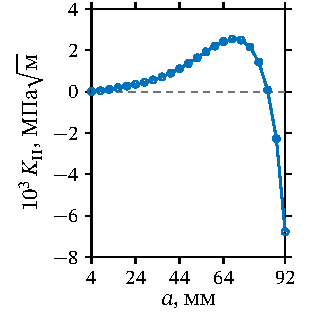
\includegraphics[width=\linewidth]{figures/intensities/KII.pdf}
    \caption{КІН поперечного зсуву $K_{\mathrm{II}}$.}
    \label{fig:intensities-KII}
  \end{subfigure}\hfill
  \begin{subfigure}[t]{0.315\linewidth}
    \centering
    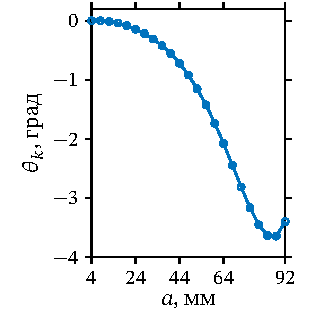
\includegraphics[width=\linewidth]{figures/intensities/theta.pdf}
    \caption{Абсолютний кут нахилу $\theta_k$.}
    \label{fig:intensities-theta}
  \end{subfigure}

  \end{minipage}
  \caption{КІН нормального відриву й поперечного зсуву (МПа$\sqrt{\text{м}}$) та кут нахилу ланки (у градусах) залежно від
накопиченої довжини тріщини $a$ (мм) за одиничного віддаленого навантаження. Кут нахилу ланки
сягає мінімуму в $P_{22}$ і стає менш від’ємним у $P_{23}$.}
  \label{fig:intensities}
\end{figure}


\subsection{Зміна знака коефіцієнта змішаності мод і зміна напряму повороту}
У $P_{21}$ ($a=84$ мм) коефіцієнт змішаності мод ще додатний:
$q_{\mathrm{K}}^{(21)}=+8.134267\times10^{-5}$. У $P_{22}$ ($a=88$ мм) він стає від’ємним:
$q_{\mathrm{K}}^{(22)}=-0.0021416$. Отже, зміна знака відбувається між двома незалежно розв’язаними прийнятими станами,
в жодному з яких коефіцієнт змішаності не дорівнює нулю. Для позначки на рис.~\ref{fig:trajectory-late} і \ref{fig:late} лінійна
інтерполяція між цими значеннями дає
\begin{equation}
 a_{\mathrm{LS}}=a_{21}
 -\frac{\qmix^{(21)}}{\qmix^{(22)}-\qmix^{(21)}}(a_{22}-a_{21})
 \simeq\LSLengthMM\ \text{мм}.\label{eq:zeroestimate}
\end{equation}
Тут $a_{\mathrm{LS}}$ позначає лише інтерпольовану оцінку довжини тріщини, за якої настала б локальна симетрія
($K_{\mathrm{II}}=0$). Розв’язку для стану з нульовою модою II не отримано. Інтерполяція не встановлює фізичного
положення з точністю, меншою за приріст довжини.

Зміна знака безпосередньо позначається на напрямі. У $P_{21}$ поворот за MTS у бік $P_{22}$ ще відбувається
за годинниковою стрілкою, тоді як від’ємний коефіцієнт змішаності в $P_{22}$ спричиняє поворот проти
годинникової стрілки до прийнятої ланки з вершиною $P_{23}$ (рис.~\ref{fig:late}). Для останнього
розв’язаного стану $K_{\mathrm{I}}=1.2444$, $K_{\mathrm{II}}=-0.0067803$ і $q_{\mathrm{K}}=-0.0054488$. Критерій MTS тоді дає $\Delta\theta_{24}=0.62435^\circ$ і $\theta_{24}=-2.7762^\circ$. Цей останній прогноз задає
продовження, геометрія якого пройшла перевірку. Прийнятого пружного розв’язку у вершині $P_{24}$
немає.

\begin{table}[htbp]\centering\small\setlength{\tabcolsep}{3.5pt}
\caption{Характерні прийняті стани. КІН наведено в МПа$\sqrt{\text{м}}$, кути — у градусах. Рядок інтерполяції містить
лише графічну оцінку нуля, без розв’язаного поля напружень або визначеного напряму тріщини.}
\begin{tabular}{lrrrrrr}\toprule
Стан & $a$ [мм] & $K_{\mathrm{I}}$ & $K_{\mathrm{II}}$ & $K_{\mathrm{II}}/K_{\mathrm{I}}$ & $\theta_k$ & $\Delta\theta_{k+1}$\\\midrule
\CharacteristicRows
Інтерполяція & \LSLengthMM & --- & --- & $0$ & --- & ---\\
\bottomrule\end{tabular}\label{tab:states}
\end{table}

\begin{figure}[htbp]
  \centering
  \begin{minipage}{0.8\textwidth}
  \centering
  \begin{subfigure}[t]{0.485\linewidth}
    \centering
    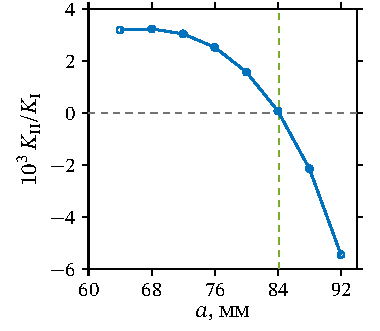
\includegraphics[width=\linewidth]{figures/late/mode_mixity.pdf}
    \caption{Змішаність мод на кінцевій ділянці.}
    \label{fig:late-mixity}
  \end{subfigure}\hfill
  \begin{subfigure}[t]{0.485\linewidth}
    \centering
    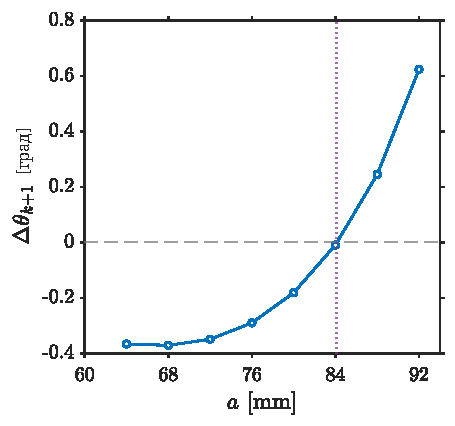
\includegraphics[width=\linewidth]{figures/late/turn.pdf}
    \caption{Покроковий поворот за MTS.}
    \label{fig:late-turn}
  \end{subfigure}

  \end{minipage}
  \caption{Зміна знака коефіцієнта змішаності мод і зміна напряму повороту за MTS. Пунктир позначає
інтерпольований нуль коефіцієнта змішаності. Кут, обчислений у $P_{23}$ ($a=92$ мм), визначає
запропоновану наступну ланку, для якої фізичного розв’язку немає.}
  \label{fig:late}
\end{figure}
\FloatBarrier


\subsection{Порівняння з COD і чутливість до способу визначення КІН}
Оскільки зміна знака коефіцієнта змішаності мод змінює напрям повороту за MTS, важливо
перевірити, чи зберігається вона за іншого способу визначення КІН. Усі вісім апроксимацій COD
дають $q_{\mathrm{K}}>0$ у $P_{21}$ та $q_{\mathrm{K}}<0$ у $P_{22}$, що узгоджується з інтервалом зміни знака за EDI. Кількісні відмінності
залежать від інтервалу апроксимації та степеня апроксимувального полінома (рис.~\ref{fig:cod}). Серед 176 апроксимацій
найбільша абсолютна різниця між кутами повороту за MTS, визначеними за COD та EDI, становить $\MaxCODError^\circ$
у $P_{23}$ для лінійної апроксимації на $[0.12,0.30]\Delta a$. Квадратичні апроксимації COD у цьому стані дають кути від
$\CODQuadMin^\circ$ до $\CODQuadMax^\circ$, тоді як за EDI одержано $0.62435^\circ$.

Поблизу локальної симетрії важливо розрізняти знак і величину малого коефіцієнта змішаності мод.
У $P_{21}$ лінійна апроксимація на найвіддаленішому від вершини інтервалі дає відношення, на $\CODNearZeroPercent$\%
більше за оцінку EDI, хоча відповідна різниця кутів повороту становить лише $\CODNearZeroTurnDiff^\circ$. Відносна
розбіжність, отже, чутлива до малого знаменника в порівнянні. Обидва способи дають той самий
інтервал зміни знака, проте спільний розв’язок для переміщень унеможливлює незалежне оцінювання
скінченно-елементної похибки. Відмінності між апроксимаціями COD характеризують чутливість до
екстраполяції й не є мірою статистичної невизначеності.

\begin{figure}[htbp]
  \centering
  \begin{minipage}{0.8\textwidth}
  \centering
  \begin{subfigure}[t]{0.485\linewidth}
    \centering
    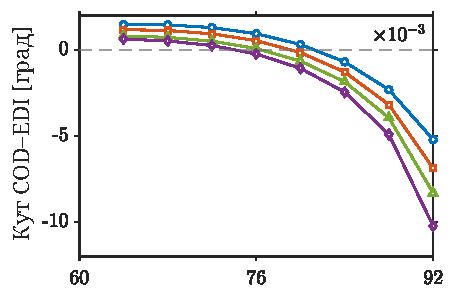
\includegraphics[width=\linewidth]{figures/cod/turn_linear.pdf}
    \caption{Різниці кутів повороту для лінійних апроксимацій COD.}
    \label{fig:cod-turn-linear}
  \end{subfigure}
  \hfill
  \begin{subfigure}[t]{0.485\linewidth}
    \centering
    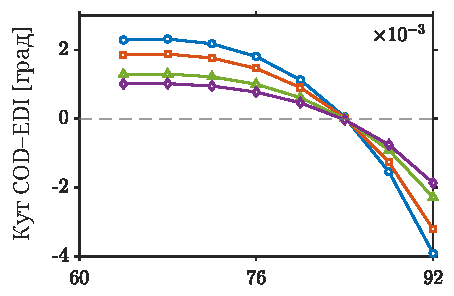
\includegraphics[width=\linewidth]{figures/cod/turn_quadratic.pdf}
    \caption{Різниці кутів повороту для квадратичних апроксимацій COD.}
    \label{fig:cod-turn-quadratic}
  \end{subfigure}

  \medskip

  \begin{subfigure}[t]{0.485\linewidth}
    \centering
    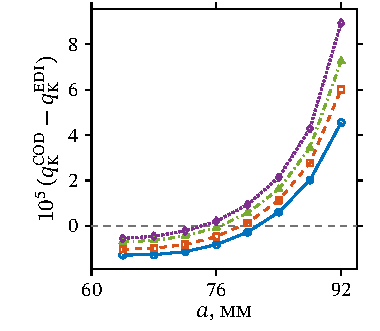
\includegraphics[width=\linewidth]{figures/cod/mixity_linear.pdf}
    \caption{Різниці коефіцієнта змішаності мод для лінійних апроксимацій COD.}
    \label{fig:cod-mixity-linear}
  \end{subfigure}
  \hfill
  \begin{subfigure}[t]{0.485\linewidth}
    \centering
    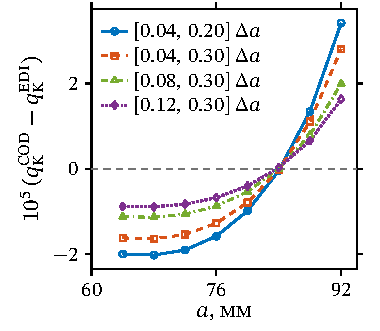
\includegraphics[width=\linewidth]{figures/cod/mixity_quadratic.pdf}
    \caption{Різниці коефіцієнта змішаності мод для квадратичних апроксимацій COD.}
    \label{fig:cod-mixity-quadratic}
  \end{subfigure}

  \end{minipage}
  \caption{Різниці COD--EDI на кінцевій ділянці траєкторії для чотирьох нормованих інтервалів апроксимації
COD та лінійної або квадратичної екстраполяції. На верхніх панелях порівняно кути повороту за
MTS, на нижніх — коефіцієнти змішаності мод. Нуль означає збіг двох способів визначення, а не
відомий точний розв’язок.}
  \label{fig:cod}
\end{figure}
\FloatBarrier


\subsection{Чутливість до деталізації структурованої сітки біля вершини}
У порівняннях за однакових довжин тріщини $\delta x$ і $\delta y$ позначають різниці координат між порівнюваною
та базовою траєкторіями, $\delta r=(\delta x^2+\delta y^2)^{1/2}$ — відстань між відповідними вершинами, а $\delta\theta$ — різницю абсолютних
кутів у фіксованій системі координат. Позначення $\Delta\theta_{k+1}$ зберігаємо для локального кута повороту за
MTS. Різниці коефіцієнта змішаності мод та інтерпольованої довжини в точці зміни знака позначено
відповідно $\delta q_{\mathrm{K}}$ і $\delta a_{\mathrm{LS}}$.

Для фіксованих прийнятих геометрій тріщини розглянуто дві особливості зміни коефіцієнта
змішаності мод. У додатному максимумі $P_{17}$ зменшення кроку структурованої сітки від $0.027012$ до $0.013506$ мм
змінює $K_{\mathrm{I}}$ на $0.00134\%$, $q_{\mathrm{K}}$ — на $1.05\times10^{-6}$, а кут повороту за MTS — на $-1.20\times10^{-4}$ градуса. Ці малі відмінності
зумовлено різною дискретизацією тієї самої фізичної геометрії.

Чутливішою є перевірка інтервалу зміни знака наприкінці траєкторії. У табл.~\ref{tab:tipmesh} порівняно поля в
$P_{21}$ і $P_{22}$ для трьох рівнів деталізації, що охоплюють чотириразову зміну $h_{\mathrm{tip}}$. На кожному з
досліджених рівнів $q_{\mathrm{K}}$ додатний в $P_{21}$ та від’ємний в $P_{22}$. Отже, інтервал і відповідна зміна напряму
повороту за MTS зберігаються за дослідженого згущення сітки біля вершини.

\begin{table}[htbp]
\centering
\small
\setlength{\tabcolsep}{2.6pt}
\caption{Чутливість до структурованої привершинної сітки для фіксованих геометрій $P_{21}$ та $P_{22}$ за спільних
радіусів області інтегрування та заданого закону розмірів зовнішніх елементів. Наведені значення
$a_{\mathrm{LS}}$ — інтерпольовані оцінки положення зміни знака. Незалежних розв’язків для станів із нульовою
модою II немає.}
\label{tab:tipmesh}
\begin{tabular}{lrrrrrr}
\toprule
Крок сітки & $h_{\rm tip}$ [мм] & $q_{\mathrm{K}}(P_{21})$ & $\Delta\theta_{22}$ [град] & $q_{\mathrm{K}}(P_{22})$ & $\Delta\theta_{23}$ [град] & $a_{\rm LS}$ [мм]\\
\midrule
$2h_0$ & 0.054025 & $+7.7957\times10^{-5}$ & $-0.008933$ &
$-2.1451\times10^{-3}$ & $+0.245805$ & 84.14027\\
$h_0$ & 0.027012 & $+8.1343\times10^{-5}$ & $-0.009321$ &
$-2.1416\times10^{-3}$ & $+0.245406$ & 84.14637\\
$h_0/2$ & 0.013506 & $+8.3031\times10^{-5}$ & $-0.009515$ &
$-2.1399\times10^{-3}$ & $+0.245207$ & 84.14941\\
\bottomrule
\end{tabular}
\end{table}

Лінійно інтерпольована оцінка $a_{\mathrm{LS}}$ змінюється від $84.14027$ мм для $2h_0$ через $84.14637$ мм для $h_0$ до $84.14941$ мм для $h_0/2$.
Послідовні зміщення на $6.10$ і $3.04~\text{мкм}$ дають орієнтовний коефіцієнт зменшення, що відповідає оцінному порядку близько $1.00$. Цей показник описує чутливість до сітки саме
\emph{інтерпольованої оцінки}. Він не характеризує збіжності розв’язку для точки з нульовою модою II. Оскільки використані фізичні стани розділяє
приріст довжини 4 мм, малі зміщення не означають, що положення локальної симетрії встановлено з
мікрометровою точністю.

Розрахунок поширення з привершинною сіткою $2h_0$ дає траєкторію, яку в масштабі зразка майже
неможливо відрізнити від траєкторії $h_0$ (рис.~\ref{fig:tipres-trajectory}). Найбільша різниця вертикальних координат
становить $0.12760~\text{мкм}$, а найбільша евклідова відстань між відповідними вершинами — $0.12800~\text{мкм}$. Обидва максимуми
припадають на $P_{23}$. Найбільша абсолютна різниця напрямів становить $0.24539$ міліградуса в $P_{22}$ (рис.~\ref{fig:tipres-dy} та
\ref{fig:tipres-dtheta}).

\begin{figure}[!t]
  \centering
  \captionsetup[subfigure]{justification=raggedright,singlelinecheck=false}
  \begin{minipage}{\textwidth}
  \centering

  \begin{subfigure}[t]{0.94\linewidth}
    \centering
    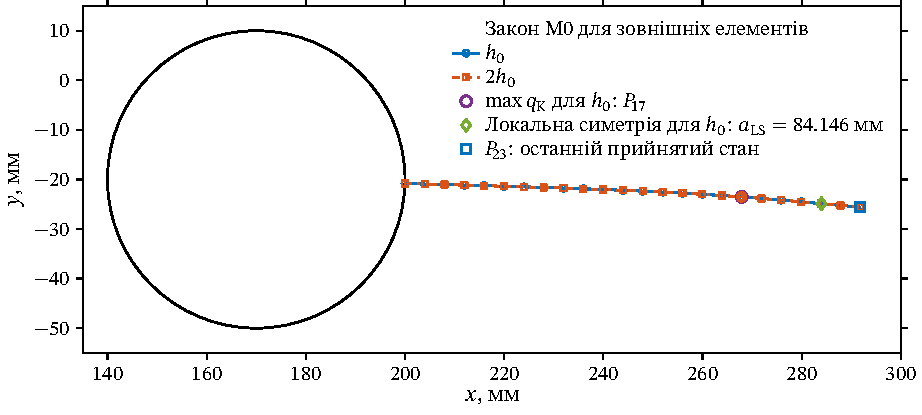
\includegraphics[width=\linewidth]{figures/tip_resolution_sensitivity/trajectory.pdf}
    \caption{Траєкторії для кроків структурованої привершинної сітки $h_0$ і $2h_0$.}
    \label{fig:tipres-trajectory}
  \end{subfigure}

  \par\smallskip

  \begin{subfigure}[t]{0.315\linewidth}
    \centering
    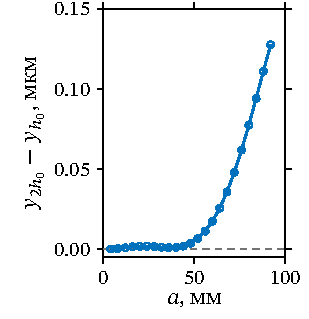
\includegraphics[width=\linewidth]{figures/tip_resolution_sensitivity/vertical_deviation.pdf}
    \caption{Різниця вертикальних координат вершин, $y_{2h_0}-y_{h_0}$.}
    \label{fig:tipres-dy}
  \end{subfigure}
  \hfill
  \begin{subfigure}[t]{0.315\linewidth}
    \centering
    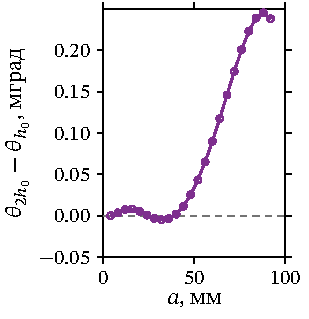
\includegraphics[width=\linewidth]{figures/tip_resolution_sensitivity/direction_deviation.pdf}
    \caption{Різниця напрямів тріщини, $\theta_{2h_0}-\theta_{h_0}$.}
    \label{fig:tipres-dtheta}
  \end{subfigure}
  \hfill
  \begin{subfigure}[t]{0.315\linewidth}
    \centering
    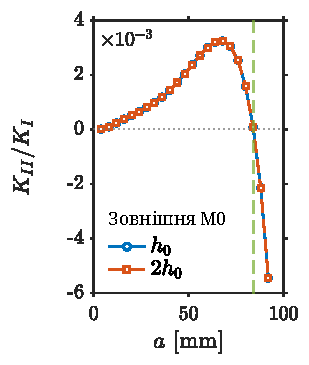
\includegraphics[width=\linewidth]{figures/tip_resolution_sensitivity/mode_mixity.pdf}
    \caption{Зміна коефіцієнта змішаності мод для двох кроків привершинної сітки.}
    \label{fig:tipres-q}
  \end{subfigure}

  \end{minipage}
  \caption{Вплив деталізації структурованої привершинної сітки на траєкторію поширення. Траєкторії $h_0$ і $2h_0$
мають спільні радіуси області інтегрування та закон M0 для зовнішніх елементів. На панелі~(d)
показано $K_{\mathrm{II}}/K_{\mathrm{I}}$. Ромб позначає інтерпольований нуль коефіцієнта змішаності мод для траєкторії $h_0$.}
  \label{fig:tip-resolution-sensitivity}
\end{figure}

У двох незалежно обчислених траєкторіях також зберігаються додатний максимум коефіцієнта
змішаності мод у $P_{17}$ і зміна його знака між $P_{21}$ та $P_{22}$ (рис.~\ref{fig:tipres-q}). Найбільша різниця $q_{\mathrm{K}}$ становить
$2.65\times10^{-7}$. Лінійна інтерполяція в інтервалах $P_{21}$--$P_{22}$ для двох незалежно обчислених траєкторій дає $a_{\mathrm{LS}}=84.14637$ мм
для $h_0$ та $84.146276$ мм для $2h_0$, тобто різницю $-0.000094$ мм ($-0.094~\text{мкм}$). Як і вище, це показник чутливості в межах
одного приросту, який не встановлює фізичного положення локальної симетрії з мікрометровою
точністю.

Додатний максимум коефіцієнта змішаності мод, інтервал зміни його знака та зміна напряму
повороту зберігаються на досліджених рівнях деталізації структурованої сітки як за фіксованих
геометрій, так і вздовж розрахованої траєкторії $2h_0$. Висновок стосується зазначених змін сітки.
При перебудові структурованої області також змінюється зв’язність узгодженої зовнішньої сітки.

\Needspace{5\baselineskip}
\subsection{Чутливість до густоти зовнішньої сітки}
Збільшення розмірів елементів зовнішньої сітки мало впливає на КІН фіксованих геометрій $P_{17}$ та
$P_{22}$. Тому його вплив на всю траєкторію перевірено розрахунком поширення на сітці M1 від спільної
першої ланки $P_0P_1$. Усі подальші напрями визначено з розв’язків M1, незалежно від траєкторії M0.

У масштабі зразка дві траєкторії майже збігаються (рис.~\ref{fig:m1mesh-trajectory}). Малу відстань між ними видно з
різниць координат і кутів на рис.~\ref{fig:m1-mesh-sensitivity}. Найбільша різниця вертикальних координат становить $0.06734~\text{мкм}$,
найбільша евклідова відстань між відповідними вершинами — $0.06742~\text{мкм}$, а найбільша абсолютна різниця
напрямів — $0.07304$ міліградуса, або $7.30\times10^{-5}$ градуса (рис.~\ref{fig:m1mesh-dy} та \ref{fig:m1mesh-dtheta}).

Характерна послідовність зберігається і при збільшенні розмірів зовнішніх елементів. На обох
розрахованих траєкторіях додатний максимум коефіцієнта змішаності мод припадає на $P_{17}$ ($a=68$ мм).
Коефіцієнт додатний у $P_{21}$ і від’ємний у $P_{22}$ (рис.~\ref{fig:m1mesh-q}). Найбільша абсолютна різниця для $q_{\mathrm{K}}$
становить $2.89\times10^{-7}$. Лінійна інтерполяція у відповідних інтервалах $P_{21}$--$P_{22}$ дає $a_{\mathrm{LS}}=84.14637$ мм для M0 і $84.146$ мм
для M1, тобто різницю $0.000322$ мм ($0.322~\text{мкм}$). Цю різницю в межах одного приросту наведено лише як показник
чутливості. Жодне інтерпольоване значення не має фізичної точності в масштабі мікрометра.

\begin{samepage}
Характерна послідовність зберігається за дослідженого збільшення розмірів елементів \emph{зовнішньої} сітки.
Оскільки привершинну дискретизацію та радіуси області інтегрування не змінювали, це порівняння
не встановлює незалежності результату від сітки загалом.
\end{samepage}

\begin{figure}[htbp]
  \centering
  \captionsetup[subfigure]{justification=raggedright,singlelinecheck=false}
  \begin{minipage}{\textwidth}
  \centering

  \begin{subfigure}[t]{0.94\linewidth}
    \centering
    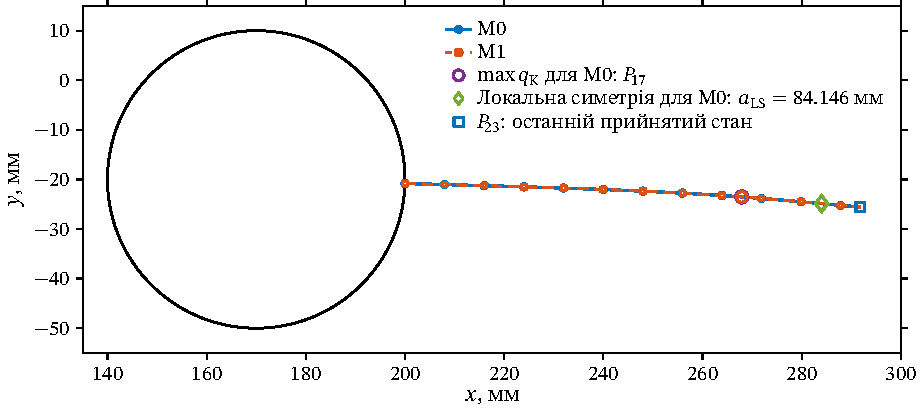
\includegraphics[width=\linewidth]{figures/m1_mesh_sensitivity/trajectory.pdf}
    \caption{Траєкторії поширення тріщини за законами M0 і M1 для розмірів зовнішніх елементів.}
    \label{fig:m1mesh-trajectory}
  \end{subfigure}

  \par\smallskip

  \begin{subfigure}[t]{0.315\linewidth}
    \centering
    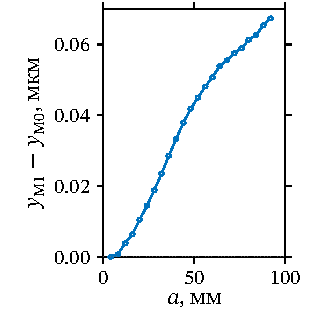
\includegraphics[width=\linewidth]{figures/m1_mesh_sensitivity/vertical_deviation.pdf}
    \caption{Різниця вертикальних координат вершин, $y_{\mathrm{M1}}-y_{\mathrm{M0}}$.}
    \label{fig:m1mesh-dy}
  \end{subfigure}
  \hfill
  \begin{subfigure}[t]{0.315\linewidth}
    \centering
    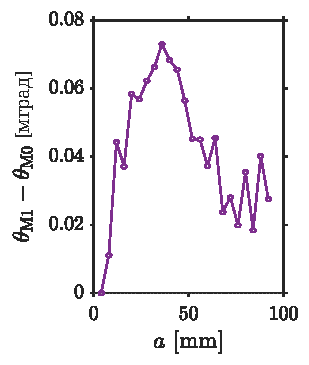
\includegraphics[width=\linewidth]{figures/m1_mesh_sensitivity/direction_deviation.pdf}
    \caption{Різниця напрямів тріщини, $\theta_{\mathrm{M1}}-\theta_{\mathrm{M0}}$.}
    \label{fig:m1mesh-dtheta}
  \end{subfigure}
  \hfill
  \begin{subfigure}[t]{0.315\linewidth}
    \centering
    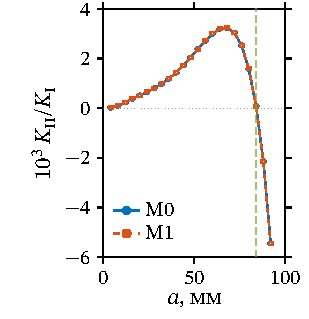
\includegraphics[width=\linewidth]{figures/m1_mesh_sensitivity/mode_mixity.pdf}
    \caption{Зміна коефіцієнта змішаності мод для M0 і M1.}
    \label{fig:m1mesh-q}
  \end{subfigure}

  \end{minipage}
  \caption{Вплив збільшення розмірів зовнішніх елементів на траєкторію тріщини. Траєкторії M0 і M1
обчислено окремо за однакової привершинної дискретизації та однакових радіусів області
інтегрування. На панелі~(d) наведено $K_{\mathrm{II}}/K_{\mathrm{I}}$. Ромб позначає інтерпольований нуль коефіцієнта
змішаності мод для траєкторії M0.}
  \label{fig:m1-mesh-sensitivity}
\end{figure}
\FloatBarrier

\subsection{Спільне зменшення приросту довжини тріщини та уточнення дискретизації}
Траєкторії для $\Delta a=4$, 2 і 1 мм майже збігаються до довжини 92 мм (рис.~\ref{fig:inc-trajectory}). Водночас різниці
положень вершин і напрямів ланок зменшуються з уточненням (рис.~\ref{fig:increment-sensitivity}). У цій серії сітку біля
вершини, область інтегрування й характерні розміри зовнішньої сітки зменшують разом з $\Delta a$, як
описано в розділі~\ref{sec:numerics}. Отже, порівняння стосується спільної зміни приросту та дискретизації.

\begin{figure}[htbp]
  \centering
  \captionsetup[subfigure]{justification=raggedright,singlelinecheck=false}
  \begin{minipage}{\textwidth}
  \centering

  \begin{subfigure}[t]{0.94\linewidth}
    \centering
    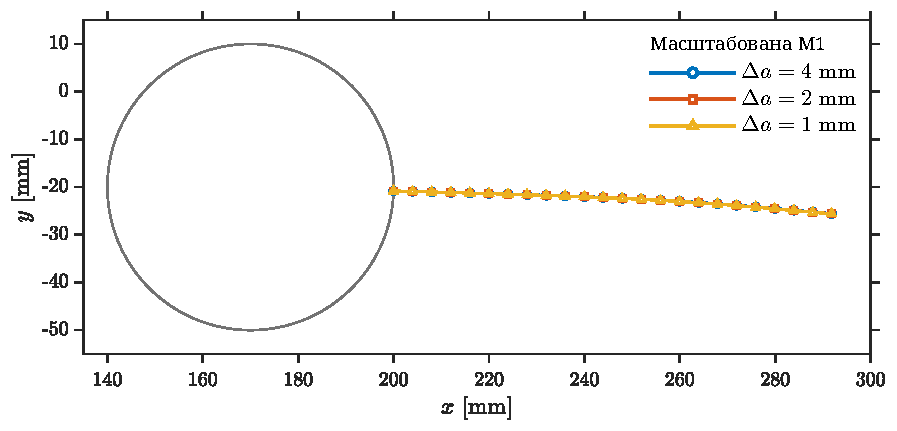
\includegraphics[width=\linewidth]{figures/increment_sensitivity/trajectory.pdf}
    \caption{Незалежно обчислені траєкторії для $\Delta a=4$, 2 і 1 мм. Кожну продовжено до 92 мм.}
    \label{fig:inc-trajectory}
  \end{subfigure}
  \par\smallskip
  \begin{subfigure}[t]{0.315\linewidth}
    \centering
    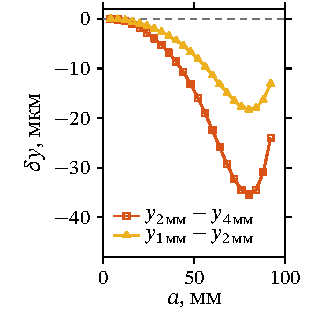
\includegraphics[width=\linewidth]{figures/increment_sensitivity/vertical_deviation.pdf}
    \caption{Послідовні різниці вертикальних координат вершин.}
    \label{fig:inc-dy}
  \end{subfigure}
  \hfill
  \begin{subfigure}[t]{0.315\linewidth}
    \centering
    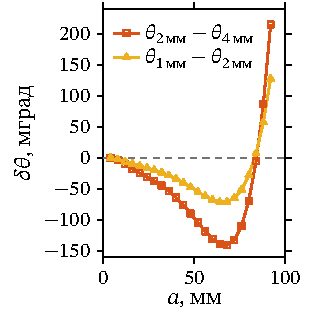
\includegraphics[width=\linewidth]{figures/increment_sensitivity/direction_deviation.pdf}
    \caption{Послідовні різниці напрямів тріщини.}
    \label{fig:inc-dtheta}
  \end{subfigure}
  \hfill
  \begin{subfigure}[t]{0.315\linewidth}
    \centering
    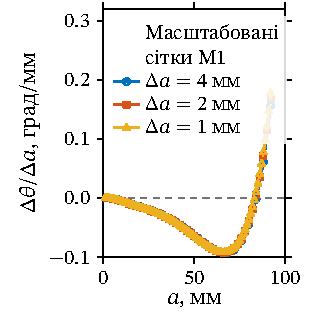
\includegraphics[width=\linewidth]{figures/increment_sensitivity/turn_density.pdf}
    \caption{Інтенсивність повороту вздовж трьох траєкторій.}
    \label{fig:inc-turn-density}
  \end{subfigure}

  \end{minipage}
  \par\medskip
  \caption{Спільне зменшення приросту довжини й уточнення дискретизації. Траєкторії з приростами $4$, $2$ і
$1$ мм мають спільні безрозмірні масштаби сітки й області інтегрування в серії масштабованих
сіток M1. На панелі~(b) показано $y_{2\,\text{мм}}-y_{4\,\text{мм}}$ і $y_{1\,\text{мм}}-y_{2\,\text{мм}}$ за точних спільних довжин тріщини. На панелі~(c)
наведено відповідні різниці абсолютних напрямів у фіксованій системі координат точки зародження.
На панелі~(d) наведено інтенсивність повороту $\Delta\theta/\Delta a$ за розрахункових довжин кожної траєкторії.}
  \label{fig:increment-sensitivity}
\end{figure}
\FloatBarrier

У табл.~\ref{tab:increment-pairwise} порівняно положення вершин і напрями за довжин тріщини, спільних для всіх трьох
траєкторій. Максимальна відстань між вершинами зменшується від $35.472~\text{мкм}$ у порівнянні 4 і 2 мм до $18.291~\text{мкм}$
у порівнянні 2 і 1 мм. Відповідні вертикальні різниці зменшуються від $35.418$ до $18.263~\text{мкм}$, а
найбільша абсолютна різниця напрямів — від $214.931$ до $127.391$ міліградуса.

\begin{table}[htbp]
\centering
\small
\setlength{\tabcolsep}{4.0pt}
\caption{Послідовні різниці між незалежно обчисленими траєкторіями в серії зі зменшенням приросту довжини
за спільних безрозмірних параметрів. Порівняння виконано за точних спільних довжин тріщини без
інтерполяції траєкторій.}
\label{tab:increment-pairwise}
\begin{tabular}{lrrrr}
\toprule
Порівняння & $\max|\delta y|$ [мкм] & $\max\delta r$ [мкм] & $\max|\delta\theta|$ [мград] & $\max|\delta q_{\mathrm{K}}|$\\
\midrule
2 мм $-$ 4 мм & 35.4181 & 35.4721 & 214.931 & $2.48578\times10^{-3}$\\
1 мм $-$ 2 мм & 18.2629 & 18.2911 & 127.391 & $1.41618\times10^{-3}$\\
\bottomrule
\end{tabular}
\end{table}

Відношення послідовних різниць становлять 1.939 для найбільшої відстані між вершинами та 1.687 для
найбільшої різниці напрямів. Якщо $d$ позначає максимум послідовної різниці, показник $p=\log_2(d_{\Delta a}/d_{\Delta a/2})$ дорівнює
приблизно 0.96 і 0.75 відповідно. Ці показники не є формальними порядками Річардсона. Порівнювані
траєкторії одержано рекурентним оновленням геометрій, максимуми можуть припадати на різні
довжини тріщини, а приріст і масштаби дискретизації змінюються одночасно. Наведені значення
описують зменшення різниць у серії з трьох рівнів і не визначають асимптотичних швидкостей
збіжності.

Доповнює цю картину зміна нормованого коефіцієнта змішаності мод. Як видно з табл.~\ref{tab:increment-characteristic}, додатний
максимум $q_{\mathrm{K}}$ зменшується від $3.23937\times10^{-3}$ за 4 мм до $1.61266\times10^{-3}$ за 2 мм і $8.04068\times10^{-4}$ за 1 мм. Попри майже пропорційне
зменшення, відношення максимуму до $\Delta a$ змінюється лише приблизно на $0.71\%$ між найгрубішим та
найдрібнішим рівнями. Відповідна інтенсивність повороту за MTS лежить у межах від $-0.092799$ до $-0.092139$
град/мм. Залежності інтенсивності повороту на рис.~\ref{fig:inc-turn-density} подібні на відповідних сітках довжин
тріщини, хоча це не встановлює збіжності до кривини гладкої граничної траєкторії.

\begin{table}[tbp]
\centering
\small
\setlength{\tabcolsep}{3.6pt}
\caption{Характерні величини для серії зі зменшенням приросту довжини тріщини. Положення локальної
симетрії оцінено лінійною інтерполяцією між двома розв’язаними станами по різні боки від $q_{\mathrm{K}}=0$.}
\label{tab:increment-characteristic}
\begin{tabular}{rrrrrr}
\toprule
$\Delta a$ [мм] & $a(q_{\mathrm{K},\max})$ [мм] & $q_{\mathrm{K},\max}$ &
\shortstack[c]{$q_{\mathrm{K},\max}/\Delta a$\\{}[мм$^{-1}$]} &
\shortstack[c]{$(\Delta\theta/\Delta a)_{q_{\max}}$\\{}[град/мм]} &
$a_{\rm LS}$ [мм]\\
\midrule
4 & 68 & $3.2394\times10^{-3}$ & $8.0984\times10^{-4}$ &
$-0.092799$ & 84.148913\\
2 & 66 & $1.6127\times10^{-3}$ & $8.0633\times10^{-4}$ &
$-0.092398$ & 83.550120\\
1 & 66 & $8.0407\times10^{-4}$ & $8.0407\times10^{-4}$ &
$-0.092139$ & 83.268112\\
\bottomrule
\end{tabular}
\end{table}

Додатний максимум зафіксовано при $a=68$ мм для траєкторії з приростом 4 мм і при $a=66$ мм для двох
траєкторій з меншими приростами. Отже, ці значення не відповідають одній довжині тріщини. Проте
їхнє майже пропорційне зменшення разом із $\Delta a$ і відносна сталість інтенсивності повороту
узгоджуються з умовним зв’язком кривини та критерію MTS у рівнянні~\eqref{eq:curvature-mts}. Спостережену поведінку
можна подати як
\begin{equation}
 q_{\mathrm{K}}=O(\Delta a),\qquad
 \Delta\theta=O(\Delta a),
 \label{eq:increment-scaling}
\end{equation}
у межах дослідженої чисельної серії. Три рівні одночасного зменшення приросту довжини та масштабів дискретизації свідчать на користь такої
залежності від масштабу. Самостійного доведення асимптотичної збіжності вони не дають.

Зміщення оцінки місця зміни знака коефіцієнта змішаності мод також зменшується за послідовного
уточнення. Лінійна інтерполяція дає $a_{\mathrm{LS}}=84.148913$, $83.550120$ і $83.268112$ мм для трьох рівнів. Послідовні різниці
становлять $0.59879$ і $0.28201$ мм. Відношення цих різниць — 2.12, а відповідний оцінний порядок — близько 1.09.
На траєкторії з приростом 1 мм знак змінюється між розв’язаними станами за довжин 83 та 84 мм.
Жодна з інтерпольованих оцінок не є розв’язаним станом з нульовим $K_{\mathrm{II}}$.

\begin{samepage}
Майже пропорційне зменшення ненормованих максимумів коефіцієнта змішаності й відносна сталість
величин, віднесених до приросту довжини, узгоджуються з умовним зв’язком MTS і кривини в
рівнянні~\eqref{eq:curvature-mts}. За наявними даними для трьох рівнів існування єдиної гладкої граничної траєкторії
не встановлено.
\end{samepage}

\Needspace{5\baselineskip}
\section{Обговорення}
\label{sec:discussion}
\subsection{Механічна інтерпретація зміни напряму повороту}
Напрям повороту кожної нової ланки визначається коефіцієнтом змішаності мод у поточній вершині
за критерієм MTS. У прийнятій системі знаків додатний $q_{\mathrm{K}}$ дає поправку за годинниковою стрілкою.
Коли $q_{\mathrm{K}}$ стає від’ємним, поправка спрямована проти годинникової стрілки. Додатний максимум
коефіцієнта змішаності мод у $P_{17}$ і подальша зміна знака між $P_{21}$ та $P_{22}$ пояснюють зміну напряму
повороту вздовж прийнятої траєкторії. Водночас $K_{\mathrm{I}}$ зростає за незмінного одиничного віддаленого
навантаження. Зміна напряму повороту відображає зміну відносного внеску поперечного зсуву. При
цьому КІН нормального відриву не зменшується, а напрям переміщення вершини по вертикалі не
змінюється на протилежний.

Залишкова горизонтальна перемичка становить лише $\LastLigamentMM$ мм у $P_{23}$. Це дає підставу припускати, що
наближення до вільного від навантаження правого краю може впливати на змішаність мод на кінцевій
ділянці. У цих розрахунках цей вплив неможливо відокремити від збільшення довжини та зміни
геометрії тріщини. Для визначення його внеску потрібне контрольоване порівняння за різних
відстаней до межі. Обчислені КІН встановлюють механізм повороту за MTS, однак не визначають
єдиної фізичної причини зміни самих КІН.

\subsection{Чисельна чутливість та інтерпретація гладкої траєкторії}
Верифікаційні дослідження стосуються різних джерел невизначеності. На заданих асимптотичних
полях перевіряють реалізацію визначення КІН. Апроксимація COD та інтеграл взаємодії дають дві
оцінки за тим самим скінченно-елементним полем переміщень. Їхній збіг поблизу зміни знака
коефіцієнта змішаності підтверджує визначений напрям повороту, однак не дає незалежної перевірки
пружного розв’язку. Перевірка для центрального отвору також підтверджує очікувану дзеркальну
симетрію та малу величину відхилення напряму на одному кроці. Вона не означає, що збурені траєкторії
наближатимуться до незбуреної на всій довжині.

За незалежними розрахунками поширення перевірено, чи змінюють відмінності дискретизації
рекурентну побудову траєкторії. При збільшенні розмірів зовнішніх елементів за законом M1
збережено попарно симетричну привершинну область і набір елементів інтегрування. При зміні кроку
структурованої привершинної сітки її узгоджена перебудова може змінити зв’язність зовнішньої
сітки навіть за незмінного заданого закону розмірів її елементів. Обидві альтернативні
траєкторії зберігають додатний максимум коефіцієнта змішаності та інтервал $P_{21}$--$P_{22}$ зміни його
знака. Найбільші відстані між відповідними вершинами, $0.0674$ та $0.128~\text{мкм}$ відповідно, малі порівняно з
приростами довжини. Це свідчить про малу чутливість до двох досліджених змін сітки. Незалежності
від усіх параметрів дискретизації ці спостереження не встановлюють.

Траєкторії з приростами 4/2/1 мм дають змогу оцінити інший аспект алгоритму. У цій серії
одночасно зменшуються приріст довжини тріщини, крок структурованої привершинної сітки, радіуси
області інтегрування та масштаби зовнішньої сітки. Послідовні різниці положень вершин і напрямів
зменшуються, а додатний максимум $q_{\mathrm{K}}$ спадає приблизно пропорційно $\Delta a$. Віднесений до приросту
максимум і відповідна інтенсивність повороту залишаються відносно сталими. Отже, розклад MTS для
малої змішаності мод дає можливий зв’язок зі знаковою кривиною гладкої граничної траєкторії
(рівняння~\eqref{eq:curvature-mts}), за умови існування такої границі й збіжності дискретних інтенсивностей повороту.
Ці три рівні одночасного зменшення приросту довжини та масштабів дискретизації не дають формального порядку збіжності та не визначають
окремого внеску похибки від приросту. Ця особливість також обмежує пряме порівняння з роботами,
де змінюють лише приріст довжини, зокрема з дворівневим порівнянням Фана та ін.~\cite{FangEtAl2020}.

У табл.~\ref{tab:independent-sensitivity} зіставлено результати зміни зовнішньої та структурованої привершинної сіток. Більші
різниці, спостережені в серії з одночасним зменшенням приросту довжини та масштабів дискретизації 4/2/1 мм, не дають змоги виокремити внесок
жодного з характерних масштабів дискретизації.

\begin{table}[htbp]
\centering
\small
\setlength{\tabcolsep}{4.2pt}
\caption{Чутливість траєкторії до деталізації зовнішньої та структурованої привершинної сіток. Різниці $a_{\mathrm{LS}}$
визначено між лінійно інтерпольованими нулями коефіцієнта змішаності в межах від $P_{21}$ до $P_{22}$.}
\label{tab:independent-sensitivity}
\begin{tabular}{lrrrrr}
\toprule
Зміна сітки & $\max|\delta y|$ [мкм] & $\max\delta r$ [мкм] &
\shortstack[c]{$\max|\delta\theta|$\\{}[мград]} &
$\max|\delta q_{\mathrm{K}}|$ & $\delta a_{\rm LS}$ [мкм]\\
\midrule
Грубіша зовнішня M1 & 0.06734 & 0.06742 & 0.07304 & $2.89\times10^{-7}$ & $-0.322$\\
Привершинна $2h_0$ & 0.12760 & 0.12800 & 0.24539 & $2.65\times10^{-7}$ & $-0.094$\\
\bottomrule
\end{tabular}
\end{table}
\FloatBarrier

У подальших перевірках слід змінювати радіуси області інтегрування, зберігаючи фізичну геометрію
тріщини та решту чисельних параметрів. Наявні перевірки якості сітки, нев’язок і заданих полів
встановлюють допустимість чисельних розрахунків, проте не дають всеохопної оцінки похибки
фізичних КІН або траєкторії. Попередній тест для довжини 8 мм збережено як перевірку визначення
КІН. До серії з одночасним зменшенням приросту довжини та масштабів дискретизації він не входить.

\subsection{Останній прийнятий стан і межі фізичної постановки}
Прийнята послідовність станів закінчується в $P_{23}$. Запропоноване продовження $P_{23}P_{24}$ пройшло перевірки
геометрії та заданих полів, але спроба розв’язати пружну задачу для тріщини довжиною 96 мм не
задовольнила критерію нев’язки PCG. Таке завершення розрахунку не можна тлумачити як фізичну
зупинку тріщини або її контакт із правим краєм.

Модель розглядає одну активну тріщину в однорідній лінійно-пружній пластині й визначає лише
напрями заданих квазістатичних приростів. Умова зародження за напруженням не задає порога подальшого поширення. Розрахунок не визначає навантажень і швидкостей поширення
чи умов зупинки. Розгалуження, конкурентне зародження, пластичність і динамічне руйнування також
виходять за межі постановки. Розрахована траєкторія не виключає цих процесів.

\section{Висновки}
\label{sec:conclusions}
За покроковою процедурою лінійної механіки руйнування визначено траєкторію однієї тріщини від контуру кругового отвору, зміщеного відносно центра пластини. Поле напружень для отвору без тріщини визначає точку зародження,
а задана перша ланка вздовж нормалі від отвору в матеріал формує початкову геометрію. Усі
наступні напрями визначають за критерієм MTS із використанням КІН у поточній вершині, обчислених
за інтегралом взаємодії. У кожній пружній задачі зберігається вся попередня траєкторія. Послідовність розв’язків, що задовольняють критерії чисельної прийнятності, з приростом 4 мм сягає 92 мм. Для наступної геометрії, що пройшла перевірки,
прийнятого фізичного розв’язку немає.

Уздовж траєкторії спостерігається характерна зміна співвідношення мод деформування. Поки $K_{\mathrm{I}}$
зростає за незмінного еталонного навантаження, додатний коефіцієнт змішаності мод сягає
максимуму в $P_{17}$, а потім змінює знак між $P_{21}$ та $P_{22}$. Пов’язана з цим зміна напряму повороту за MTS
зменшує модуль від’ємного нахилу останньої прийнятої ланки. Розрахунки встановлюють цей механізм
зміни напряму без виокремлення внеску наближення до вільної межі.

Чисельні порівняння підтверджують збереження цих характерних особливостей за досліджених змін
привершинної та зовнішньої сіток. Перевірка для центрального отвору підтверджує очікувану зміну напряму на одному кроці за дзеркальної симетрії. Стійкості всієї траєкторії вона не встановлює. У
серії незалежно обчислених траєкторій з приростами 4/2/1 мм геометричні й кутові різниці
зменшуються, якщо одночасно зменшувати приріст і характерні розміри дискретизації. Майже
пропорційне зменшення ненормованого коефіцієнта змішаності мод і відносна сталість мір повороту,
віднесених до приросту, узгоджуються з умовною інтерпретацією гладкої траєкторії. Проте це не доводить збіжності до неперервної граничної траєкторії.

Результати стосуються вибору напряму в рамках лінійної механіки руйнування за заданих
квазістатичних приростів без критерію поширення чи зупинки тріщини. Для розмежування впливу
чисельного визначення КІН та фізичних причин зміни напряму на кінцевій ділянці доцільно
перевірити чутливість до області інтегрування й виконати контрольовані порівняння за різних
відстаней до межі.

\FloatBarrier
\section*{Декларації}
\noindent\textbf{Фінансування.}
Роботу виконано в межах базового фінансування Інституту механіки ім. С. П. Тимошенка НАН
України. Окремого дослідницького гранту для цієї роботи не надано.
\appendix
\section{Параметри чисельного методу та його верифікація}
\label{app:numerical-details}
\paragraph{Параметри дискретизації.}
Для основної траєкторії використано такі безрозмірні параметри:
\[
 \frac{h_{\mathrm{tip}}}{\Delta a}=0.00675308135,\quad
 \frac{r_{\mathrm{core}}}{\Delta a}=0.75,\quad
 \frac{r_{\mathrm{in}}}{\Delta a}=0.10,\quad
 \frac{r_{\mathrm{out}}}{\Delta a}=0.65.
\]
За приросту 4 мм крокам привершинної сітки $2h_0$, $h_0$ і $h_0/2$ відповідають
3318, 12678 і 49518 трикутних елементів структурованої області. Числові значення
цих кроків становлять 0.054025, 0.027012 і 0.013506 мм відповідно.
Для сітки з кроком $h_0$ носій вагової функції охоплює 11316 елементів.
У сітці на рис.~\ref{fig:mesh-levels} градієнт вагової функції не дорівнює тотожно нулю
в 10278 із цих елементів, а в решті 1038 елементів функція дорівнює одиниці.
Для M0 і M1 верхня межа розміру віддалених елементів становить відповідно 2.5 і 5 мм,
нахил функції зміни розміру --- 0.10 і 0.15, параметр зростання граничної метрики --- 0.25 і 0.35.
Довжина перехідної ділянки в обох випадках становить 4 мм.
Для тріщин довжини 68 та 88 мм перехід від M0 до M1 за незмінної геометрії тріщини
зменшує загальну кількість
елементів T3 на 31--33\%, а кількість зовнішніх елементів --- на 40--43\%.
Привершинна область і носій вагової функції зберігаються.

У серії з приростами 4, 2 та 1 мм безрозмірний крок привершинної сітки вдвічі більший за основний,
відносні радіуси незмінні. Для зовнішньої сітки за безрозмірним законом M1 використовуємо
\[
 \frac{h_{\mathrm{far}}}{\Delta a}=1.25,\qquad
 \frac{L_{\mathrm{tr}}}{\Delta a}=1.00,
\]
де $h_{\mathrm{far}}$ --- максимальний заданий розмір віддаленого елемента, $L_{\mathrm{tr}}$ ---
довжина перехідної ділянки. Нахил функції зміни розміру та параметр зростання граничної метрики
становлять 0.15 і 0.35. Траєкторії порівнюємо за спільних довжин 4, 8, \ldots, 92 мм без інтерполяції.
Довжину тріщини, за якої коефіцієнт змішаності мод змінює знак, оцінюємо лінійною
інтерполяцією між двома сусідніми розрахунковими значеннями, без окремого розв’язання
задачі для цієї довжини.

\paragraph{Обчислення КІН.}
Градієнти фактичного поля переміщень обчислюємо за функціями форми T6, допоміжні напруження
беремо з асимптотичних полів, а похідні допоміжних переміщень обчислюємо центральними
скінченними різницями з кроком
\[
 h=\max(10^{-7}\ \text{м},10^{-5}r).
\]
Для інтегрування застосовуємо 16-точкову квадратуру на трикутнику. Для COD використовуємо
щонайменше 12 пар вузлів у кожному з чотирьох інтервалів апроксимації. Для рівнів $2h_0$, $h_0$
і $h_0/2$ кількості пар становлять відповідно (19, 28, 23, 18), (38, 55, 44, 34) і (74, 108, 86, 67).
Для сітки з кроком $4h_0$ кількості пар становлять (10, 15, 12, 9).
Через недостатню кількість вузлів у першому та четвертому інтервалах цю сітку
не використовуємо для зіставлення КІН та кутів повороту. Інтервали апроксимації
перекриваються.

\paragraph{Якість сітки та точність розв’язання системи рівнянь.}
Під час побудови сітки забезпечуємо відповідність межам області, роздільність вузлів берегів
тріщини, спільність вузлів перед вершиною, узгодженість сітки та додатність площ елементів
і якобіанів перетворення координат.
Найменший допустимий кут трикутника становить $20^\circ$, а найбільше допустиме відношення
найдовших сторін сусідніх елементів --- 1.8.
Систему рівнянь для вільних ступенів вільності симетризуємо, застосовуємо симетричне наближене
впорядкування за мінімальним степенем та метод спряжених градієнтів із симетричним
передобумовленням Гаусса--Зейделя (PCG із SGS).
Допуск нев’язки PCG становить $10^{-10}$, максимальна кількість ітерацій --- 5000,
допуск незалежно перерахованої фактичної відносної нев’язки --- $5\times10^{-10}$.
На дрібніших сітках за фіксованої геометрії допускаємо один перезапуск PCG з отриманого
наближення без зміни системи рівнянь, передобумовлення або допусків нев’язки.
Задані переміщення виконуються точно.

Для заданих асимптотичних полів чистих мод і слабко змішаного випадку з одиничним КІН
нормального відриву та зсувним КІН $10^{-4}$ допуск відносної похибки відновлення становить
$2\times10^{-4}$; допуски паразитного внеску іншої моди й суперпозиції --- $10^{-10}$.
Для основної траєкторії розв’язки із заданими допусками нев’язки отримано до довжини тріщини 92 мм.
За довжини 96 мм, незважаючи на задовільну якість сітки та точність визначення КІН за
заданими полями, заданих допусків розв’язання крайової задачі не досягнуто.
Для довжин тріщини від 8 до 92 мм найбільша фактична відносна нев’язка становить близько
$\MaxTrueResidual$, кількість ітерацій PCG --- 2442--3011.

\paragraph{Перевірка симетрії.}
Для центрального отвору використано ті самі габарити, радіус отвору, привершинну дискретизацію,
метод EDI та розв’язувач. Центр отвору має координати $(0.150,0)$ м, перша радіальна ланка
завдовжки 4 мм з’єднує точки $(0.180,0)$ та $(0.184,0)$ м.
Для п’яти заданих напрямів другої ланки прогнозований напрям третьої наведено
в табл.~\ref{tab:symmetric-stability}.
\begin{table}[htbp]
\centering
\small
\caption{Задані та прогнозовані напрями ланок тріщини для центрального отвору.}
\label{tab:symmetric-stability}
\begin{tabular*}{0.64\linewidth}{@{\extracolsep{\fill}}rr}
\toprule
$\theta_2$, град & $\theta_3$, град\\
\midrule
$-0.10$ & $+0.011415$\\
$-0.05$ & $+0.005708$\\
$0$     & $-7.13\times10^{-7}$\\
$+0.05$ & $-0.005708$\\
$+0.10$ & $-0.011415$\\
\bottomrule
\end{tabular*}
\end{table}
КІН нормального відриву є наближено парною функцією заданого збурення, а коефіцієнт змішаності
та прогнозований напрям третьої ланки --- наближено непарними.
Позначимо відображення напрямів через $F(\theta_2)=\theta_3$.
Симетричні скінченно-різницеві оцінки нахилу становлять $-0.11416$ і $-0.11415$;
апроксимація методом найменших квадратів із проходженням через початок координат дає
\[
 F'(0)\approx-0.11415.
\]
Це оцінка для одного кроку; на наступних кроках змінюється вся геометрія тріщини,
тому отримане відображення не можна застосовувати повторно як незмінне.

\paragraph{Показники якості сітки та розв’язку.}
На рис.~\ref{fig:quality} наведено характеристики якості сітки та точності розв’язання
системи рівнянь залежно від довжини тріщини. Ці характеристики не є оцінками похибки
дискретизації траєкторії.
\begin{figure}[htbp]
  \centering
  \begin{minipage}{0.8\textwidth}
  \centering
  \begin{subfigure}[t]{0.485\linewidth}
    \centering
    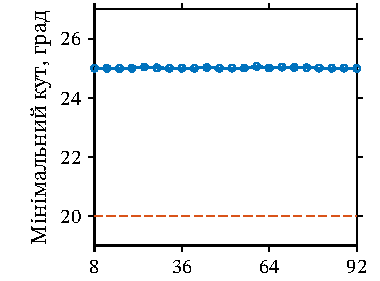
\includegraphics[width=\linewidth]{figures/quality/min_angle.pdf}
    \caption{Найменший кут трикутника.}
    \label{fig:quality-angle}
  \end{subfigure}
  \hfill
  \begin{subfigure}[t]{0.485\linewidth}
    \centering
    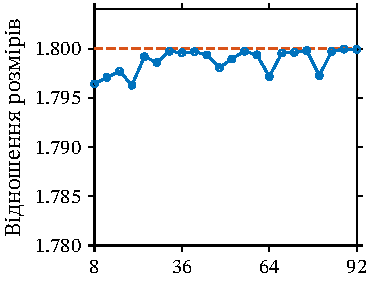
\includegraphics[width=\linewidth]{figures/quality/size_ratio.pdf}
    \caption{Відношення розмірів сусідніх елементів.}
    \label{fig:quality-ratio}
  \end{subfigure}

  \medskip

  \begin{subfigure}[t]{0.485\linewidth}
    \centering
    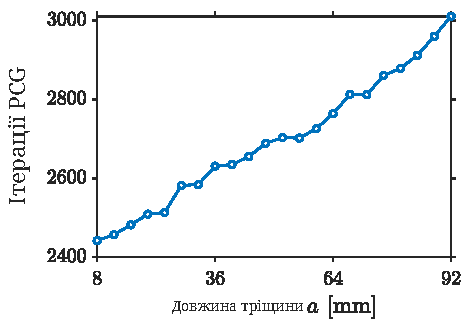
\includegraphics[width=\linewidth]{figures/quality/iterations.pdf}
    \caption{Кількість ітерацій PCG.}
    \label{fig:quality-iterations}
  \end{subfigure}
  \hfill
  \begin{subfigure}[t]{0.485\linewidth}
    \centering
    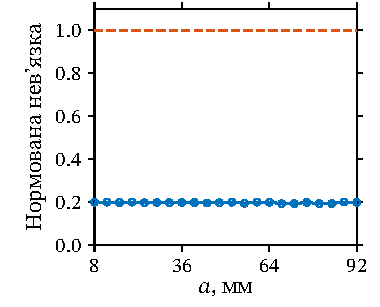
\includegraphics[width=\linewidth]{figures/quality/true_residual.pdf}
    \caption{Нормована відносна нев’язка.}
    \label{fig:quality-residual}
  \end{subfigure}

  \end{minipage}
  \caption{Характеристики сітки та розв’язання системи рівнянь для тріщин довжини від 8 до 92 мм.
Штрихові лінії відповідають допустимим значенням: мінімальний кут $20^\circ$,
максимальне відношення розмірів сусідніх елементів 1.8 і одиничне значення відносної нев’язки,
нормованої на $5\times10^{-10}$. Допуск нев’язки PCG становить $10^{-10}$.}
  \label{fig:quality}
\end{figure}

\FloatBarrier
\begin{english}
\small
\raggedright
\setlength{\bibsep}{3pt}
\renewcommand{\refname}{Література}
\bibliographystyle{unsrtnat}
\bibliography{references}
\end{english}


\end{document}
